\documentclass[
12pt, % Баримтын фонтын хэмжээ, сонголт: 10pt, 11pt, 12pt
oneside, % Хоёр талаар хэвлэж үдэхээр тохируулсан. Нэг тал бол комментыг арилга
%chapterinoneline,% Нэг мөрөнд бүлгийн дугаар, нэрийг гаргах
english, % babel багцын хэлний тохиргоо
onehalfspacing, % Мөр хоорондын зай. Сонголтууд: singlespacing, onehalfspacing, doublespacing
%draft, % Ноорог горимд шилжихийн тулд комментыг арилга(зураг, холбоос, hboxes гарахгүй)
nolistspacing, % Хэрэв мөр хоорондын зай onehalfspacing эсвэл doublespacing бол, жагсаалтын мөр хоорондын зайг single болгохын тулд комментыг арилга
%liststotoc, % Зураг/хүснэгт/бусад жагсаалтыг гарчигт оруулахын тулд комментыг арилга
%toctotoc, % Uncomment to add the main table of contents to the table of contents
%parskip, % Параграф хооронд зай оруулахын тулд комментыг арилга
%nohyperref, % hyperref багцыг ачаалахгүй бол комментыг арилга
headsepline, % Толгой мөрийн доогуур шугам татахын тулд комментыг арилга
]{MUST-Thesis} % Энэ класс файл нь баримтын бүтцийг тодорхойлно

\usepackage[utf8]{inputenc} % Олон улсын тэмдэгт оруулахад хэрэгтэй
\usepackage[T2A]{fontenc} % Олон улсын тэмдэгтийн гаралтын кодчилол
\usepackage[mongolian]{babel}

\usepackage{titlesec}
\usepackage[table]{xcolor}
\usepackage{rotating} % эргүүлэх
\usepackage{enumitem}
\let\oldtabular\tabular
\let\endoldtabular\endtabular
\renewenvironment{tabular}
{\bgroup\singlespacing\oldtabular}%
{\endoldtabular\egroup}
\let\oldverse\verse
\let\endoldverse\endverse
\renewenvironment{verse}
{\bgroup\singlespacing\oldverse}%
{\endoldverse\egroup}

\usepackage{caption,longtable,ltcaption}
\DeclareCaptionJustification{nohyphen}{\hyphenpenalty=10000}
\captionsetup{justification=nohyphen}

\usepackage{pgf}
\usepackage{tikz} % зураг зурах
\usetikzlibrary{shapes,arrows,automata}

\definecolor{OliveGreen}{cmyk}{0.64,0,0.95,0.40}
\definecolor{CadetBlue}{cmyk}{0.62,0.57,0.23,0}
\definecolor{Cover}{RGB}{102,255,255}
\definecolor{Chapter}{RGB}{255,220,180}

\definecolor{lightlightgray}{gray}{0.9}
\usepackage{listings}
\renewcommand{\lstlistingname}{Эх код} % Програмын эх код хэвлэх
\lstset{
	language=C,                             % Code langugage
	basicstyle=\linespread{1.0}\ttfamily,                   % Code font
	keywordstyle=\color{OliveGreen},        % Keywords font ('*' = uppercase)
	commentstyle=\color{CadetBlue},         % Comments font
	numbers=left,                           % Line nums position
	numberstyle=\tiny,                      % Line-numbers fonts
	stepnumber=1,                           % Step between two line-numbers
	numbersep=5pt,                          % How far are line-numbers from code
	backgroundcolor=\color{lightlightgray}, % Choose background color
	frame=none,                             % A frame around the code
	tabsize=2,                              % Default tab size
	captionpos=t,                           % Caption-position = bottom
	breaklines=true,                        % Automatic line breaking?
	breakatwhitespace=false,                % Automatic breaks only at whitespace?
	showspaces=false,                       % Dont make spaces visible
	showtabs=false,                         % Dont make tabls visible
	columns=flexible,                       % Column format
	morekeywords={__global__, __device__},  % CUDA specific keywords
}

\usepackage[autostyle=false]{csquotes} % Ном зүйд хэлнээс хамаарсан хашилт оруулахад хэрэгтэй

\usepackage[backend=bibtex,natbib=true,sorting=none,sortcites]{biblatex} % Ном зүйд bibtex -г ашиглах

\addbibresource{references.bib} % Ном зүйн файл

\newcommand{\authorshipname}{Зохиогч эрхийн хамгаалал}
\newcommand{\abbrevname}{Товчилсон үгс}
\newcommand{\constantsname}{Физик тогтмолууд}
\newcommand{\symbolsname}{Таних тэмдэгтүүд}
\newcommand{\acknowledgementname}{Талархал}
\newcommand{\abstractname}{Хураангуй}

%-------------------------------------------------------------------------------
%	THESIS INFORMATION
%-------------------------------------------------------------------------------

\thesistitle{Хичээлийн материал оруулах} % Таны ажлын нэр, нүүр болон хураангуй хуудсанд ашигласан. Өөр газарт бол \ttitle командыг хэрэглэнэ
\thesistype{Бакалаврын төгсөлтийн ажил} % Удирдагчийн нэр, нүүр хуудсанд ашиглана. Дурын газарт бол \thesisname командыг хэрэглэнэ
\supervisor{Магистр. Б.Золбоо} % Удирдагчийн нэр, нүүр хуудсанд ашиглана. Дурын газарт бол \supname командыг хэрэглэнэ
\reader{Доктор(PhD) Д.Ганбат } % Шүүмжлэгчийн нэр, Дурын газарт бол \readname командыг хэрэглэнэ
\advisor{Магистр. Б.Золбоо} % Зөвлөгчийн нэр, Дурын газарт бол \advicename командыг хэрэглэнэ
\degreeind{D061203} % Мэргэжлийн индекс, нүүр болон хураангуй хуудсанд ашигласан. Өөр газарт бол \degreeid командыг хэрэглэнэ
\degree{Мэдээллийн систем} % Боловсролын зэрэг, нүүр болон хураангуй хуудсанд ашигласан. Өөр газарт бол \degreename командыг хэрэглэнэ
\authorshort{О.Нямсүрэн} % Таны товч нэр, нүүр болон хураангуй хуудсанд ашигласан. Дурын газарт бол \shortname командыг хэрэглэнэ 
\authorlong{Олзвойн Нямсүрэн} % Таны бүтэн нэр, нүүр болон хураангуй хуудсанд ашигласан. Дурын газарт бол \longname командыг хэрэглэнэ 
\addresses{nyamsuren030@gmail.com} % Таны хаяг, одоогоор ашиглаагүй. Өөр газарт бол \addressname командыг хэрэглэнэ
\subject{Мэдээллийн технологи} % Таны салбар, одоогоор ашиглаагүй. Дурынр газарт бол \subjectname командыг ашиглана
\keywords{Материал, Оюутан} % Түлхүүр үгс, одоогоор ашиглаагүй. Дурын газарт бол \keywordnames командыг хэрэглэнэ
\university{\href{http://www.must.edu.mn}{Шинжлэх Ухаан Технологийн Их Сургууль}} % Их сургуулийн нэр ба веб хаяг. Дурын газарт бол \univname командыг хэрэглэнэ 
\department{Мэдээллийн технологийн салбар} % Сургууль/тэнхмийн нэр, нүүр болон хураангуй хуудсанд ашигласан. Дурын газарт бол\deptname командыг хэрэглэнэ
\deptchair{Дэд проф. PhD. А.Алтангэрэл} % Тэнхим/эрхлэгчийн нэр, нүүр болон хураангуй хуудсанд ашигласан. Дурын газарт бол\chairname командыг хэрэглэнэ
\group{Робот техникийн баг} % Судалгааны баг/тэнхмийн нэр, нүүр хуудсанд ашигласан. Дурын газарт бол \groupname командыг хэрэглэнэ
\faculty{\href{http://www.sict.edu.mn}{Мэдээлэл, Холбооны Технологийн Сургууль}} % Салбар сургууль/факультетийн нэр, нүүр болон хураангуй хуудсанд ашигласан. Дурын газарт бол \facname командыг ашиглана

\hypersetup{pdftitle=\ttitle} % Pdf файлын гарчиг
\hypersetup{pdfauthor=\shortname} % Pdf файлын зохиогчийн нэр
\hypersetup{pdfkeywords=\keywordnames} % Pdf файлын түлхүүр үгс
\hypersetup{allcolors=black} % Pdf файлын бүх холбоос хар өнгөтэй

\usepackage{longtable}
\begin{document}
	
	\frontmatter % Агуулгын өмнөх хуудас дугаарлалт: i, ii, iii, iv... г.м.
	
	\pagestyle{plain} % Тезисийн загварыг дуудах хүртэлх толгой мөрийн суурь загвар
	
	%-------------------------------------------------------------------------------
%	TITLE PAGE
%-------------------------------------------------------------------------------
\pagecolor{Cover}
\begin{titlepage}
\begin{center}

{\scshape\LARGE \univname\par} % Их сургуулийн нэр
{\scshape\Large \facname\par}\vspace{0.5cm} % Их сургуулийн нэр

\begin{figure}[!htbp]
\centering

\includegraphics[scale=0.2]{figures/MUST_logo.png}
\end{figure}

\vspace{1cm}
\hfill \large{\longname} \\

\vspace{1cm}

{\huge \bfseries \ttitle\par}\vspace{0.4cm} % Тезисийн нэр

\vspace{3cm}
\textsc{\Large {\thesisname}}\\ % Тезисийн төрөл

\vfill

\large {Улаанбаатар хот} \\
{\large 2018 он}\\
 
\end{center}
\end{titlepage}
\pagecolor{white}

%-------------------------------------------------------------------------------
%	SUBTITLE PAGE
%-------------------------------------------------------------------------------

\begin{titlepage}
\begin{center}

{\scshape\LARGE \univname\par} % Их сургуулийн нэр
{\scshape\Large \facname\par}\vspace{0.5cm} % Их сургуулийн нэр

\vspace{2cm}
\hfill \large{\deptname} \\

\vspace{2cm}

{\huge \bfseries \ttitle\par}\vspace{0.4cm} % Тезисийн нэр

\vspace{2cm}

\begin{minipage}[t] {0.9\textwidth}
\begin{flushleft} 
\normalsize

Мэргэжлийн индекс: \degreeid \\
Мэргэжил: \degreename \\[2cm]

\emph{Удирдагч:} {\supname} \\% Удирдагчийн нэр
\emph{Зөвлөгч:} {\advicename} \\ % Зөвлөгч нарын нэрс
\emph{Гүйцэтгэгч:} {\shortname} \\ % Зохиогчийн нэр

\end{flushleft}
\end{minipage}

\vfill

\large {Улаанбаатар хот} \\
{\large 2018 он}\\ % Date

\end{center}
\end{titlepage}

  % Нүүр хуудас
%	%-------------------------------------------------------------------------------
%	WORK PLAN & REVIEW PAGE
%-------------------------------------------------------------------------------

\begin{titlepage}

\vspace*{0.5cm}
Батлав. \deptname ын эрхлэгч: 
\begin{flushright}
\makebox[4cm]{\dotfill} /\chairname/ 
\end{flushright}

Удирдагч: 
\begin{flushright}
\makebox[4cm]{\dotfill} /\supname/
\end{flushright}

\begin{center}

\vspace*{2cm}
\textbf{{\large ТӨГСӨЛТИЙН АЖЛЫН \\ ТӨЛӨВЛӨГӨӨ}}\\[0.5cm]

\textsc{\large Сэдэв: ''\ttitle''}\\[0.5cm]

\begin{tabular}{|c|p{7cm}|c|c|}
	%\rowcolor{gray!40}
	\hline
	№ & \makebox[7cm][c]{Ажлын бүлэг, хэсгийн нэр} & Эзлэх хувь & Дуусах хугацаа \\ \hline
	1 & {Удиртгал}         &  5\% & 2016-10-05 \\ \hline
	2 & {Онолын хэсэг}     & 25\% & 2016-10-30 \\ \hline
	3 & {Судалгааны хэсэг} & 30\% & 2016-11-15 \\ \hline
	4 & {Төслийн хэсэг}    & 30\% & 2016-12-20 \\ \hline
	5 & {Дүгнэлт}          & 10\% & 2016-12-25 \\ \hline
\end{tabular}

\vspace{2cm}
Төлөвлөгөөг боловсруулсан оюутан: \makebox[3cm]{\dotfill} /\shortname/

\end{center}

\newpage

\begin{center}

\vspace*{2cm}
\textbf{{\large ТӨГСӨЛТИЙН АЖЛЫН ЯВЦ}}\\[0.5cm]

\begin{tabular}{|c|p{7cm}|c|c|}
	%\rowcolor{gray!40}
	\hline
	№ & \makebox[7cm][c]{Хийж гүйцэтгэсэн ажил} & Биелсэн     & Удирдагчийн \\
	  &                    & хугацаа    & гарын үсэг \\ \hline
	1 & {Удиртгал}         & 2016-10-05 &  \\ \hline
	2 & {Онолын хэсэг}     & 2016-10-30 &  \\ \hline
	3 & {Судалгааны хэсэг} & 2016-11-15 &  \\ \hline
	4 & {Төслийн хэсэг}    & 2016-12-20 &  \\ \hline
	5 & {Дүгнэлт}          & 2016-12-25 &  \\ \hline
\end{tabular}

\vspace{1cm}
Ажлын товч дүгнэлт \\[0.5cm]
\dotfill \\[0.2cm]
\dotfill \\[0.2cm]
\dotfill \\[0.2cm]
\dotfill \\[0.2cm]
\dotfill \\[0.2cm]
\dotfill \\[0.2cm]
\dotfill \\[0.5cm]
Удирдагч: \makebox[3cm]{\dotfill} /\supname/ \\

\vspace{2cm}
ЗӨВШӨӨРӨЛ \\[0.5cm]
Оюутан \shortname гын бичсэн төгсөлтийн ажлыг УШК-д хамгаалуулахаар тодорхойлов.\\[0.5cm]
Салбарын эрхлэгч: \makebox[3cm]{\dotfill} /\chairname/
\end{center}

\end{titlepage}

\newpage

\begin{titlepage}
\begin{center}

{\scshape\Large \univname\par} % Их сургуулийн нэр
{\scshape\large \facname\par}\vspace{1cm} % Их сургуулийн нэр

\textbf{{\Large ШҮҮМЖИЙН ХУУДАС}}\\[1cm]

\end{center}

\normalsize

\deptname ын салбарын төгсөх курсийн оюутан \shortname -н ''\ttitle'' сэдэвт төгсөлтийн ажлын шүүмж.

\begin{enumerate}
\item Төслөөр дэвшүүлсэн асуудал, үүнтэй холбоотой онолын материал уншиж судалсан байдал. Энэ талаар хүмүүсийн хийсэн судалгаа, түүний үр дүнг уншиж тусгасан эсэх.
\begin{center}
\dotfill \\[0.1cm]
\dotfill \\[0.1cm]
\dotfill \\[0.1cm]
\dotfill \\[0.1cm]
\dotfill \\[0.1cm]
\dotfill \\[0.1cm]
\dotfill \\[0.4cm]
\end{center}
\item Төслийн ерөнхий агуулга. Шийдсэн зүйлүүд, хүрсэн үр дүн. Өөрийн санааг гарган, харьцуулалт хийн, дүгнэж байгаа чадвар.
\begin{center}
\dotfill \\[0.1cm]
\dotfill \\[0.1cm]
\dotfill \\[0.1cm]
\dotfill \\[0.1cm]
\dotfill \\[0.1cm]
\dotfill \\[0.1cm]
\dotfill \\[0.4cm]
\end{center}
\item Эмх цэгцтэй, стандарт хангасан өөрөөр хэлбэл диплом бичих шаардлагуудыг биелүүлсэн эсэх. Төсөлд анзаарагдсан алдаанууд, зөв бичгийн болон өгүүлбэр зүйн гэх мэт /Хуудас дугаарлагдаагүй, зураг хүснэгтийн дугаар болон тайлбар байхгүй, шрифт хольсон, хувилсан зүйл ихээр оруулсан/.
\begin{center}
\dotfill \\[0.1cm]
\dotfill \\[0.1cm]
\dotfill \\[0.1cm]
\dotfill \\[0.1cm]
\dotfill \\[0.1cm]
\dotfill \\[0.1cm]
\dotfill \\[0.4cm]
\end{center}
\item Төслөөр орхигдуулсан болон дутуу болсон зүйлүүд. Цаашид анхаарах хэрэгтэй зүйлүүд.
\begin{center}
\dotfill \\[0.1cm]
\dotfill \\[0.1cm]
\dotfill \\[0.1cm]
\dotfill \\[0.1cm]
\dotfill \\[0.1cm]
\dotfill \\[0.1cm]
\dotfill \\[0.4cm]
\end{center}
\item Төслийн талаар онцолж тэмдэглэх зүйлүүд.
\begin{center}
\dotfill \\[0.1cm]
\dotfill \\[0.1cm]
\dotfill \\[0.1cm]
\dotfill \\[0.1cm]
\dotfill \\[0.1cm]
\dotfill \\[0.1cm]
\dotfill \\[0.4cm]
\end{center}
\item Ерөнхий оноо. (5 оноо)
\begin{center}
\dotfill \\[1cm]
\end{center}
\end{enumerate}
Шүүмж бичсэн: \makebox[3cm]{\dotfill} /\readname/ \\[0.5cm]
Ажлын газар: \dotfill \\[0.5cm]
Хаяг (Утас) \makebox[5cm]{\dotfill}
\end{titlepage}
 % Төлөвлөгөө, гүйцэтгэл, шүүмжийн хуудас
	%-------------------------------------------------------------------------------
%	DECLARATION PAGE
%-------------------------------------------------------------------------------
\begin{declaration}
\addchaptertocentry{\authorshipname}

\noindent Миний бие \shortname, ''{\ttitle}'' сэдэвт энэ ажил нь минийх бөгөөд дараахыг нотолж байна. Үүнд:

\begin{itemize} 
\item Горилогч энэ ажлыг тус сургуулиас боловсролын зэрэг авахаар бүхэлд нь буюу голлон хийсэн болно.
\item Энэ ажлын аль нэг хэсгийг тус сургуульд эсвэл өөр байгууллагад боловсролын зэрэг, мэргэшил авахаар өмнө нь илгээсэн бол түүнийгээ тодорхой заасан болно.
\item Бусад хүмүүсийн хэвлүүлсэн ажлаас зөвлөгөө авсан бол түүнийгээ үндэслэсэн болно.
\item Бусад хүмүүсийн ажлаас ишлэл хийхдээ гол эх үүсвэрийг нь заасан болно.
\item Миний ажилд тусалсан голлох бүх эх үүсвэрт талархаж байна.
\item Ажлыг бусадтай хамтарсан бол алийг нь бусад хүмүүс хийсэн болохыг тодорхой заасан болно.
\end{itemize}
\bigskip
 
\noindent Гарын үсэг: \rule[-0.5em]{12.7em}{0.5pt}
\bigskip

\noindent Огноо: \rule[-0.5em]{15em}{0.5pt}

\end{declaration}

\clearpage

 % Мэдэгдлийн хуудас
	%%-------------------------------------------------------------------------------
%	QUOTATION PAGE
%-------------------------------------------------------------------------------

\vspace*{0.2\textheight}

\noindent\enquote{\itshape Thanks to my solid academic training, today I can write hundreds of words on virtually any topic without possessing a shred of information, which is how I got a good job in journalism.}\bigbreak

\hfill Dave Barry 
\normalfont

 % Ишлэл хуудас
	%-------------------------------------------------------------------------------
%	ABSTRACT PAGE
%-------------------------------------------------------------------------------

\addchaptertocentry{Хураангуй} % Хураангуйг гарчигт нэмэх

\begin{center}
{\scshape\Large \univname\par} % Их сургуулийн нэр
{\scshape\large \facname\par}\vspace{0.5cm} % Их сургуулийн нэр
{\huge\textbf{{Хураангуй}} \par}
\bigskip
{\Large{\ttitle} \par} % Тезисийн нэр
\bigskip

{\normalsize \shortname \par} % Зохиогчийн нэр
\addressname
\end{center}

%\textit{\textbf{Түлхүүр үгс: \keywordnames}}
\bigskip

Энэхүү төслийн хүрээнд их сургуулийн сошиал системийн модуль хэсэг "чат" веб аппликейшнийг хөгжүүлэхийг зорьсон билээ. 

Энэхүү сошиал систем нь их сургуулийн багш нар, ажилчид, оюутнуудад зориулсан бөгөөд тэдгээрийн хоорондын харилцаа, сургалтын системийг хөнгөвчлөх, дэмжих зорилготой.

Энэ ажил нь манай сургуулийн практикт тулгуурлан хийгдэж байгаа тул гаргасан загвар хэрэгцээ шаардлагыг бүрэн тусгахыг зорьсон.



 % Ажлын хураангуй
	%-------------------------------------------------------------------------------
%	ACKNOWLEDGEMENTS
%-------------------------------------------------------------------------------

\begin{acknowledgements}
\addchaptertocentry{\acknowledgementname}

Бусад хүмүүст зориулсан талархлыг энд оруулна. Удирдагчаа оруулахаа битгий мартаарай \ldots

\end{acknowledgements}

 % Талархлын хуудас
	%-------------------------------------------------------------------------------
%	ABBREVIATIONS
%-------------------------------------------------------------------------------

\begin{abbreviations}{ll} % Товчлолын жагсаалт оруулах (хоёр багатай хүснэгт)
\addchaptertocentry{\abbrevname}

\textbf{МVC} & \textbf{М}odel \textbf{V}iew \textbf{C}ontroller\\
\textbf{ПХ} & \textbf{П}рограм \textbf{Х}ангамж\\
\textbf{SQL} & \textbf{S}tructed \textbf{Q}uery \textbf{L}anguage\\
\textbf{GNU} & \textbf{G}eneral \textbf{P}ublic \textbf{License}\\
\textbf{CMS} & \textbf{C}ontent \textbf{M}anagement \textbf{S}ystem\\
\textbf{JSON} & \textbf{J}ava \textbf{S}cript \textbf{O}bject \textbf{N}otation\\
\textbf{WWW} & \textbf{W}orld \textbf{W}ide \textbf{W}eb\\
\textbf{HTML} & \textbf{H}ypertext \textbf{T}ext \textbf{M}arkup \textbf{L}anguage\\
\textbf{PHP} & \textbf{H}ypertext \textbf{P}reprocessor\\
\textbf{JS} & \textbf{J}ava \textbf{S}cript\\
\textbf{JQuery} & \textbf{J}avascript \textbf{Q}uery\\
\textbf{PDF} & \textbf{P}ortable \textbf{D}ocument \textbf{F}ormat\\
\textbf{АНУ} & \textbf{А}мерикийн \textbf{Н}эгдсэн \textbf{У}лс\\
\textbf{МТ} & \textbf{М}эдээллийн \textbf{Т}ехнологи\\
\textbf{ӨЕС} & \textbf{Ө}гөгдлийн \textbf{Е}рөнхий \textbf{С}хем\\
\end{abbreviations}

 % Товчилсон үгс
	%%----------------------------------------------------------------------------------
%	PHYSICAL CONSTANTS/OTHER DEFINITIONS
%---------------------------------------------------------------------------------
\addchaptertocentry{\constantsname}

\begin{constants}{lr@{${}={}$}l} % Физик тогтмолыг 3 баганатай хуүснэгтээр харуулах

% The \SI{}{} command is provided by the siunitx package, see its documentation for instructions on how to use it

	Гэрлийн хурд & $c_{0}$ & \SI{2.99792458e8}{\meter\per\second} \\
%Constant Name & $Symbol$ & $Constant Value$ with units\\

\end{constants}
  % Ашигласан тогтмолууд
	%%-------------------------------------------------------------------------------
%	SYMBOLS
%-------------------------------------------------------------------------------

\begin{symbols}{lll} % Таних тэмтгийн жагсаалт оруулах (гурван баганатай хүснэгт)
\addchaptertocentry{\symbolsname}

$a$ & distance & \si{\meter} \\
$P$ & power & \si{\watt} (\si{\joule\per\second}) \\
%Symbol & Name & Unit \\

\addlinespace % Ром тэмдгийг Грекээс зааглах

$\omega$ & angular frequency & \si{\radian} \\

\end{symbols}

 % Ашгласан таних тэмдгүүд
	%%-------------------------------------------------------------------------------
%	DEDICATION
%-------------------------------------------------------------------------------

\dedicatory{Өөрийн \ldots -д зориулав} 

 % Ажлыг хэнд зориулсан
	
	%-------------------------------------------------------------------------------
	%	LIST OF CONTENTS/FIGURES/TABLES PAGES
	%-------------------------------------------------------------------------------
	
	\tableofcontents % Гарчиг хэвлэх
	\listoffigures % Зургийн жагсаалт хэвлэх
%	\listoftables % Хүснэгтийн жагсаалт хэвлэх Хэрэгтэ бол сэргээх
	
	%-------------------------------------------------------------------------------
	%	THESIS CONTENT - CHAPTERS
	%-------------------------------------------------------------------------------
	
	\mainmatter % Хуудасны тоон (1,2,3...) дугаарлалт эхлэнэ
	
	\pagestyle{thesis} % Хуудасны тогойг "thesis" загвар руу буцаах
	\myformat % Бүлгийн нэрийг тусгай хуудсанд хэвлэх
	
	% Тезисийн бүлгүүдийг Chapters хавтаснаас бие даасан файл байдлаар оруулах
	
	% Бүлэг 1

\chapter{Оршил} % Бүлгийн нэр
\label{Chapter1} % Энэ бүлэг рүү ишлэл хийх бол \ref{Chapter1} командыг ашигла 

% Агуулгад ашигласан хэвшүүлэлтийн зарим командын тодорхойлолт
\newcommand{\keyword}[1]{\textbf{#1}}
\newcommand{\tabhead}[1]{\textbf{#1}}
\newcommand{\code}[1]{\texttt{#1}}
\newcommand{\file}[1]{\texttt{\bfseries#1}}
\newcommand{\option}[1]{\texttt{\itshape#1}}

%-------------------------------------------------------------------------------
\section{Зорилго}
Их дээд сургуулиудын багш нар хичээлийн материал болон лабораторын удирдамжаа онлайн байршуулах зорилготой. 

	\section{Зорилтууд}
		\begin{itemize}
			\item Хэрэглэгчийн шаардлага тодорхойлно. 
			\item Интерфэйс html хуудас.
			\item Активити диаграм, модель классын код.
			\item ERD диаграм, контролёр классын код.
			\item Класс диаграм, харуулах хуудасны код php.
			\item Дарааллын диаграм, JS кодчилол.
			\item Бичиг баримт-сорил1.
			\item Тайлан, статистик код.
			\item Модулын нэгтгэл.
			\item Зүгшрүүлэлт
			\item Програм-сорил2
		\end{itemize}
	
	\section{Үнэлгээ}
		\begin{itemize}
			\item Найдвартай
			\item Уян хатан
			\item Ашигтай (Мэтгэлцээний клуб болон гишүүд мэдээллээ цахимаар авна)
			\item Хэрэглээтэй (Компьютерийн архитектураас үл хамааран ямар ч үйлдлийн систем дээр ажиллах боломжтой)
			\item Сайжруулалттай (цаашид засвар, шинэчлэлт хийх боломжтой)
			\item Үнэлгээ 	
		\end{itemize}


%------

%-------------------------------------------------------------------------------
\section{Хөгжүүлэлтэд ашиглах алгоритм}

\LaTeX{} бол Microsoft Word, Adobe Pages шиг \textsc{WYSIWYG} (Таны Харж байгаа Зүйл бол Таны Оруулсан Зүйл) төрлийн текст боловсруулах програм биш. \LaTeX{} --д зориулсан баримт нь үнэндээ \emph{хэвшүүлээгүй} задгай текст бүхий файл юм. Өөрийн тексттэй хамт түүнийг хэрхэн хэвшүүлэхийг тухай энгийн командыг бичиж, энэ файлаар \LaTeX{} --т хэлж өгдөг. Жишээ нь \emph{текстийг налуу болгож тодотгохдоо} \verb|\emph{text}| командыг ашиглах ба налуу болгох текстээ их хаалтанд бичнэ. Өөрөөр хэлбэл \LaTeX{} нь HTML -тэй маш төстэй ''{mark-up}'' хэл юм.

%-------------------------------------------------------------------------------

\section{Технологийн судалгаа}

	\subsection{MySQL}
	
	MySQL нь холбоост өгөгдлийн санг удирдах систем юм. MySQL хэмээх нэрний хувьд уг системийг санаачлан хөгжүүлэгч Micheal Widenius-ын охины нэр My + SQL(Structed Query Language) гэсэн утгатай ажээ.
	Энэ систем нь GNU (General Public License) буюу нээлтэй эхийн систем учир хүссэн хэн бүхэн хөгжүүлэлтэнд оролцож, үнэгүй хэрэглэж болох юм. Эзэмшигч нь алдарт Java-г хөгжүүлсэн Sun MicroSystems компани байсан ба, одоогоор Sun-г Oracle корпораци эзэмших болсон билээ.
	Үнэгүй програм хангамжийн өгөгдлийн санг удирдах системд ихэвчлэн MySQL-ийг хэрэглэдэг бөгөөд тэдгээрийн сонгодог жишээ гэвэл Joomla, Drupal, Wordpress, phpBB гэх мэт агуулга удирдах системүүд (CMS-Content Management System), Wikipedia, Facebook, Google гэх мэт томоохон компаниуд хэрэглэдэг юм.
	Хөгжүүлэлт нь C/C++ хэл дээр хийгдсэн ба AIX, BSDi, FreeBSD, HP-UX, i5/OS, Linux, Mac OS X, NetBSD, Novell NetWare, OpenBSD, OpenSolaris, eComStation, OS/2 Warp, QNX, IRIX, Solaris, Symbian, SunOS, SCO OpenServer, SCO UnixWare, Sanos, Tru64, Microsoft Windows гэсэн олон үйлдлийн системүүд дээр ажилладаг.
	MySQL бол хамгийн өргөн хэрэглээтэй нээлттэй эхийн (Open Source) өгөгдлийн сан удирдах програм юм. Анх 1995 онд зах зээлд гарсан ба с/с++ хэл дээр бичигдсэн. Одоогийн байдлаар 5.7 нь хамгийн сүүлийн хувилбар болон гараад байна. Энэ сүүлийн хувилбар дээр нэмэгдсэн давуу талууд гэвэл 3 дахин хурдан үйл ажиллагаатай болсон мөн натив JSON дэмжигчтэй болсон гэх мэт шинэлэг үйлдлүүд нэмэгдсэн байна.
	
	\subsection{Php}
	  Rasmus Lerdorf WWW-д вэб хуудас үүсгэх үедээ өгөгдөл боловсруулах хялбархан арга хайж байгаад 1995 онд PHP хэлийг скрипт хэл байдлаар зохиосон.
	PHP нь сервер талын скрипт хэл ба динамик вэб хуудас хийхэд илүү тохиромжтой. Энэ скрипт хэл нь энгийн хэрэглээний вэб сайтаас эхлээд байгууллагын иж бүрэн вэб программ хийж болохоор MySQL мэтийн өгөгдлийн сантай харилцан ажиллах боломжтой.
	Хуудас ачаалах үед броузерээр нэг бүрчлэн уншдаг HTML-тэй адилгүй, PHP баримтыг бэлтгэхдээ серверээр урьдчилан боловсруулдаг. PHP код агуулсан хуудас нь хэрэглэгчийн броузерт илгээгдхээс өмнө серверээр боловсруулагдсан байдаг.
	PHP хэлний өөр нэг давуу тал бол скриптэн хэл юм. Ихэнх програмчлалын хэлнүүдэд ажиллахын өмнө машины хэл рүү хөрвүүлэх тусгай файлууд /compile/ шаардлагатай байдаг бол PHP хэлний хувьд хөрвүүлэлт хийх шаардлагагүй байдаг тул код засварлах болон шалгахад илүү хурдан байдаг
	
	\subsection{Системийн судалгаа}
	Үндэслэл
		Мэдээллийн технологийнн ололт амжилттай уялдаж дэлхийн улс орнуудад цахим сургалт нь өргөн хүрээнд хэрэгжиж байна.
		Орчин үеийн технологид суурилсан сургалтын шинэ арга хэлбэрийг ашигллан цаг хугацаа, орон зайнаас үл хамааран боловсрол олгох, насан туршийн суралцах боломжийг бий болгох зорилгыг хэрэгжүүлэхэд шийдвэл зохих тулгамдсан асуудал бол нэгдсэнн стандарт бүхий э-хичээл боловсруулах шаардлагтай байгаа юм.
		
		Э-хичээл боловсруулах стандарт байхгүй тохиолдолд багш бүр өөр өөрийн хувилбараар боловсруулах ба энэ нь цахим сургалтын үр дүнд муугаар нөлөөлнө.
		
	Стандарт гэж юу вэ? 
		Стандарт нь хэмжээ, загвар гэсэн утгатай ба өргөн утгаараа үлгэрчилсэн загвар, эх хэмжүүр, бүдүүвчилсэн зураг гэсэн утгатай үг юм. Үүнийг онлайн сургалтанд дараах байдлаар тодорхойлдог байна. 
		
		Э-хичээлийн стандарт-----------------------нийтлэг дагаж мөрдөх дүрэм журмын багц юм. 
		
	Онлайн хичээл явуулахад анхаарах техникийн шаардлагууд
	
		Сургалтанд ашиглагдах онлайн сургалтын систем нь бүх хэрэглэгчидэд хүртээмжтэй, энгийн щ, ашиглахад хялбар байх. 
		Интернэтийн хурдаас үл хамааран суралцагч гэрээсээ, сургуулиасаа аль ч үед хандаж суралцах боломжтой. 
		Нийтлэг ашиглагддаг үйлдлийн систем болох Windows болон Mac үйлдлийн системүүдийн аль алинд нь зохицож ажиллаж болдог байх.
		Видео болон аудио файлын хэмжээ нь 8MB-аас ихгүй байх.
		Текстэн материалууд нь суралцагчдад хүртээмжтэй стандарт форматаар хангагдсан байх.
		Суралцагч өөрийн компьютераасаа хичээлийн материалыг хэвлэж, хадгалж болохуйцаар агуулгад шигтэж өгсөн байх.
		Болж өгвөл үнэгүй эсвэл лицензтэй программ хангамж ашигласан байх.
		
	Дэлгэцийн зохиомждоо дараахыг анхаарах
	
		Хичээлийн текстийг дэлгэцэнд бүтнээр нт багтаа. Энэ нь уншиж боловсруулахад төхөм болно.
		Текстийн хэмжээг 5-8 мөрөөр хязгаарлаж, 15-аас дээш мөр оруулахгүй байж, 8 хүртэлх үгийг нэг мөрөнд багтаах.
		Дэлгэцэнд текстийн 1 ба 2-оос илүү хэлбэртэй параграф оруулахгүй байх.
		Хэрэглэхэд ойлгомжтой, энгийн байх(ээдрээтэй, эргэлзээтэй би).
		Өртөг зардал, цаг хугацаа хэмнэсэн байх.
		
	Дүгнэлт 
	
		Лекцийн бүтэц, технологи нь цаг үеийн шаардлагыг даган өөрчлөгдөж боловсронгуй болж байх ёстой зүйлийн нэг мөн.
		Судлаачдын тогтоосоноор лекцийн явцад оюутнуудын анхаарал 10-15 минутын давтамжтай 2-3 удаа буурдаг байна.
		Лекцийн хичээлийн чанарыг сайжруулахын тулд суралцагчдын сурах сэдлийг бий болгох явдал чухал үүрэгтэй.
		Семинар болон лабораиорын хичээл нь оюутны мэдлэгийг бататгах, гүнзгийрүүлэх, өргөжүүлэх, мэдлэгээ амьдралдаа хэрэглэх арга барил, чадвар дадал олгох үүрэг зориулалттай сургалтын зохион байгуулалтын нэг хэлбэр юм.
		\newpage
		\subsubsection{Оюутны вэб}
		\begin{figure}
			\centering
			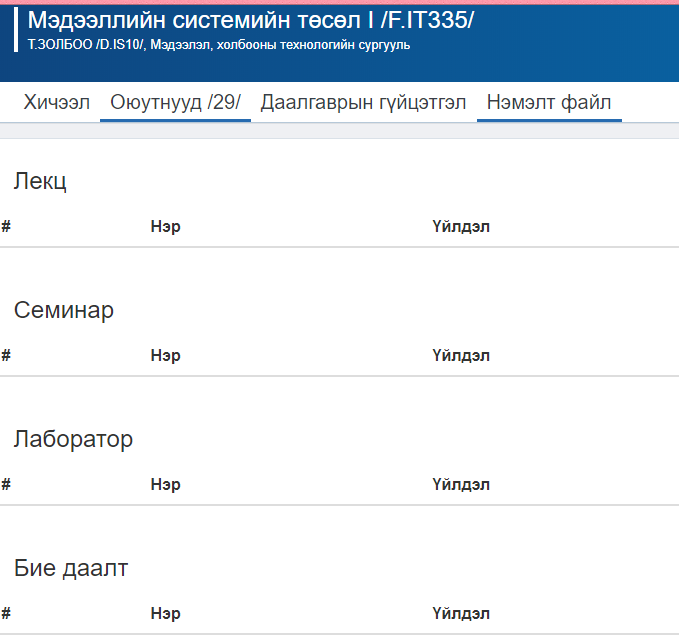
\includegraphics[scale=0.5]{Diagrams/Sudalgaa1}
			\caption[Оюутны вэб https://student.cloudmis.edu.mn/Login]{Оюутны вэб https://student.cloudmis.edu.mn/Login}
			\label{text}
		\end{figure}
	
		\newpage
		\subsubsection{ШУТИС МХТС Цахим сургалт}
		\begin{figure}
			\centering
			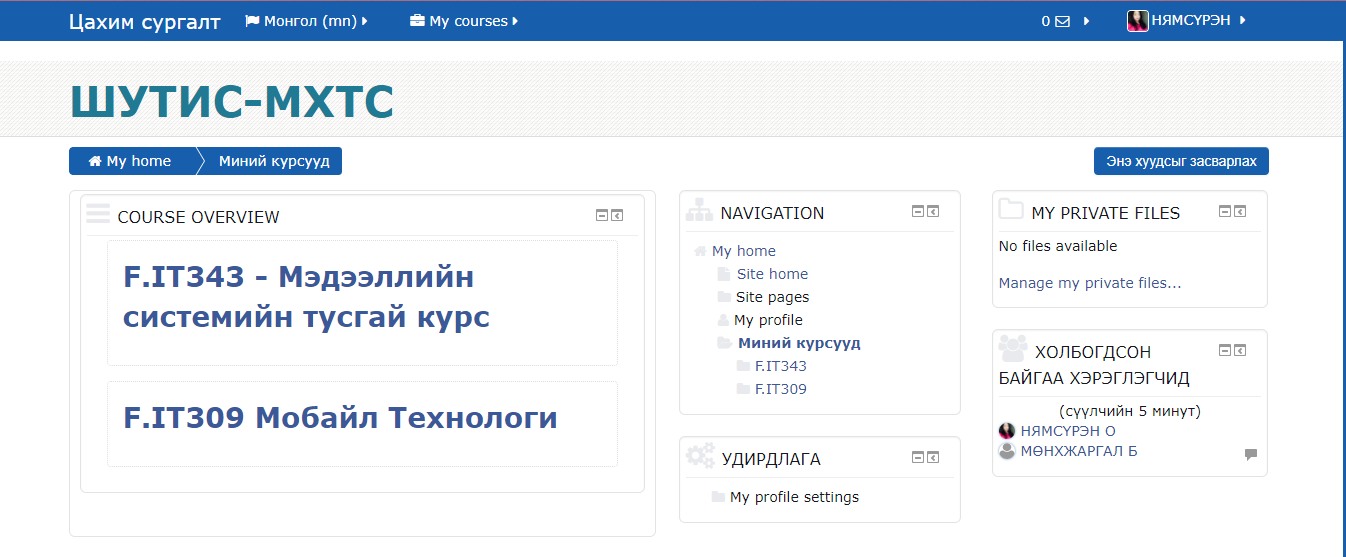
\includegraphics[scale=0.5]{Diagrams/Sudalgaa2}
			\caption[Цахим сургалт http://elearn.sict.edu.mn/login/index.php]{Цахим сургалт http://elearn.sict.edu.mn/login/index.php}
			\label{text}
		\end{figure}
		
			\newpage
		\subsubsection{ШУТИС МХТС Цахим сургалт}
		\begin{figure}
			\centering
			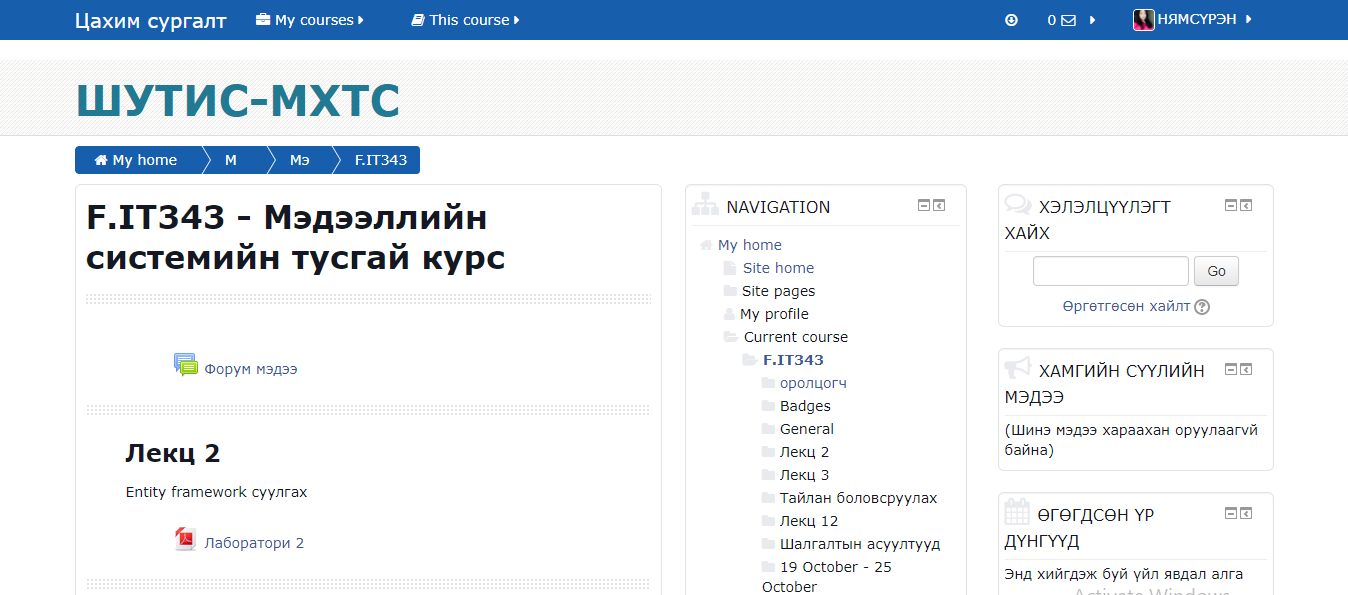
\includegraphics[scale=0.5]{Diagrams/Sudalgaa3}
			\caption[Цахим сургалт http://elearn.sict.edu.mn/login/index.php]{Цахим сургалт http://elearn.sict.edu.mn/login/index.php}
			\label{text}
		\end{figure}
\section{Бүлгийн дүгнэлт}

	Энэ бүлэгт өөрийн хийх гэж буй вэбийн зорилго зорилт болон ашиглах програмчлалын хэл болон архитектурын судалгаа, онол агуулгын мэдээллээ орууллаа.
%-------------------------------------------------------------------------------
	% Бүлэг 2

\chapter{Шаардлага, зохиомжийн бүлэг} % Бүлгийн нэр
\label{Chapter2} % Энэ бүлэг рүү ишлэл хийх бол \ref{Chapter1} командыг ашигла 

\section{Модулийн үйл ажиллагааны тухай дэлгэрэнгүй }
Энэхүү систем нь Их дээд сургуулийн багш хичээлээ улирлаар үүсгээд, тухайн хичээлийг үзэх оюутнуудыг кодоор нь нэмээд хичээлийн материалаа оруулна.

\section{Модулыг ашиглах хэрэглэгчид}
Их дээд сургуульд суралцдаг оюутан, багш.
\section{Функционал шаардлага}
 Энэхүү модул нь оюутан,багш гэсэн 2 оролцогчтой.
Багш нь: Өөрийн бүртгэлээр нэвтэрч ороод улиралаар хичээлээ үүсгэнэ, хичээлийн материалаа оруулна, тухайн хичээлийг үзэж байгаа оюутнуудыг кодоор нь нэмнэ.
Оюутан: Өөрийн бүртгэлээр нэвтэрч ороод багшийн тавьсан хичээлийн материал, даалгавар, лабораторын удирдамжийг татаж авах буюу систем дээр нээж үзэж болно.

\subsection{Багшын шаардлага}
\begin{itemize}
	
	\item Улирлаар хичээлээ үүсгэх
	\item Хичээлийн материал оруулах хичээлээ сонгох
	\item Хичээлийн материал оруулах
	\item Тухайн хичээлийг үзэж байгаа оюутнуудыг нэмэх
	\item Хайлт хийх
	
	\subsection{Оюутны шаардлага}
	\begin{itemize}
		\item Үүссэн хичээ рүү орох
		\item Хичээлийн материалаа систем дээр нээж харах болон татаж үзэх
	\end{itemize}
	
	\subsection{Системийн шаардлага}
	\begin{itemize}
		\item Тайлан гаргах
		\subitem Хамгийн их файл оруулдаг багш нарын тайланг графикаар харуулах
		\subitem Файлын тоог улирлаар харуулах
		\subitem Татагдсан файлын тоог харуулах
		\item Мэдэгдэл шидэх
	\end{itemize}
\end{itemize}
\section{Функциональ бус шаардлага}
\begin{itemize}
	\item Бүтээгдэхүүний 
	\subitem Хичээлийн материалыг систем дээр харуулах
	\subitem Системийн цагийн хуваарь 24/7 байх
	\subitem Бүх төрлийн төхөөрөмжөөс үзэхэд тохиромжтой хэлбэрээр харагддаг байх буюу загвар нь responsive байх
	
	\item Байгууллагын
	\subitem Өгөгдлийн санд өгөгдлийг нэг форматаар хадгалагддаг байх
	
	\item Гадаад
	\subitem Системд нэвтрэх эрхийг хязгаарлаж, хамгаалдаг байх
	\subitem Бусад албан байгууллагатай хамтран ажилладаг байх
\end{itemize}
\newpage
\section{Юзкейс диаграм}
	\begin{figure}[htbp]
		\centering
		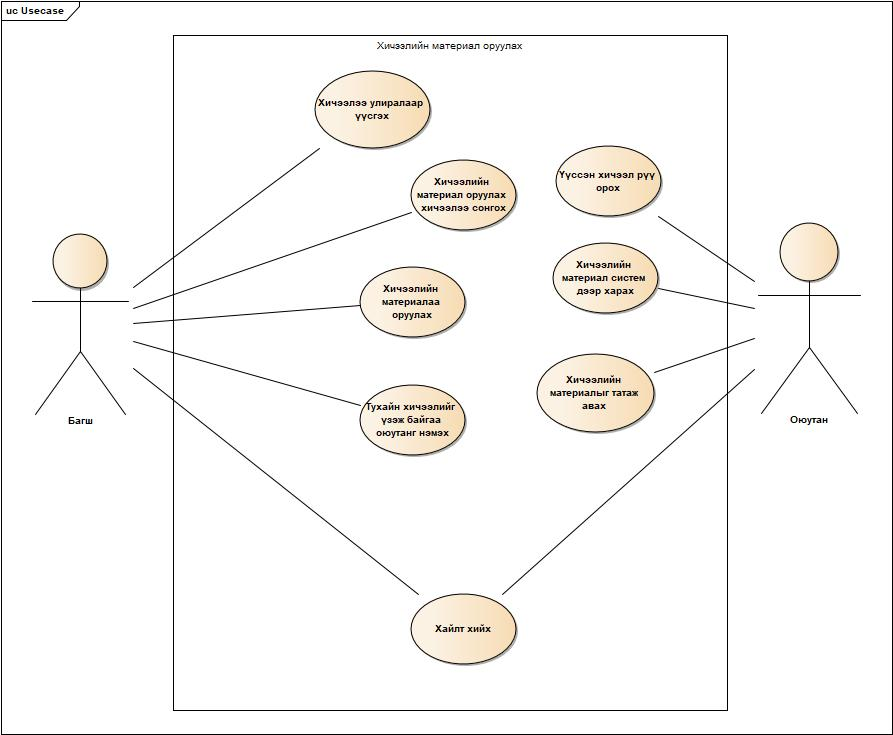
\includegraphics[scale=0.5]{Diagrams/UseCase}
		\caption[Юзкейс диаграм]{Юзкейс диаграм}
		\label{fit:UseCase}
	\end{figure}


\section{Юзкейс диаграмын тодорхойлолт}

\begin{center}
	\begin{table}[!htbp]
		\caption{}
		\begin{tabular}{|p{4cm}|p{11cm}|}
			\hline
			Нэр: & Хичээлийн материал оруулах \\
			\hline
			ID: & 1 \\
			\hline
			Товч тайлбар: & Багш шинээр хичээлээ үүсгэнэ. \\
			\hline
			Триггер: & Багш нь бүртгүүлэх шаардлагатай болсон. \\
			\hline
			Үндсэн оролцогч: & Багш \\
			\hline
			Хоёрдогч оролцогч: & Байхгүй  \\
			\hline
			Өмнөх нөхцөл: &  Веб сервер ажиллагаатай байх\\
			\hline
			Ажлын урсгал: & \begin{enumerate}
				\item Багш хичээлийн материал оруулах сонгосноор энэ юз кейс эхлэнэ. 
				\item Веб сервер нь багшид материал оруулах цонхыг харуулна. 
				\item Багш материалаа оруулна. 
				\item Веб сервер нь багшийн оруулсан мэдээллийг шалгана. 
				\item IF (“мэдээлэл үнэн зөв бол”)
				\begin{enumerate}
					\item[5.1] Веб сервер багшийн оруулсан мэдээллийг баазад хадгална.
					\item[5.2] Веб сервер багшийг амжилттай материал оруулсаныг нь харуулна. 
				\end{enumerate}
				\item ELSE
				\begin{enumerate}
					\item[6.1] Веб сервер нь багшийн оруулсан материалыг шалгана.  
					\item[6.2] Веб сервер нь алдаатай материалыг тодруулж харуулна. 
					\item[6.3] Веб сервер нь материал дахин оруулахыг асууна. 
				\end{enumerate}
			\end{enumerate}
			\\					  \hline
			Дараах нөхцөл: &
			\begin{enumerate}
				\item Багш веб серверд материал оруулсан байна. 
				\item Багшийн оруулсан материал баазад хадгалагдсан байна. 
			\end{enumerate}	   
			\\				   \hline
			Альтернатив урсгал: &  \begin{enumerate}
				\item Багш материалыг цуцалсан.
				\item Веб сервер дээр алдаа гарсан. 
			\end{enumerate}
			\\	\hline
		\end{tabular}
	\end{table}
\end{center}

\begin{center}
	\begin{table}[!htbp]
		\caption{}
		\begin{tabular}{|p{4cm}|p{11cm}|}
			\hline
			Нэр: & Хичээлээ улирлаар үүсгэх\\
			\hline
			ID: & 1 \\
			\hline
			Товч тайлбар: & Багш шинээр улирлаа үүсгэнэ. \\
			\hline
			Триггер: & Багш улирал үүсгэх шаардлагатай болсон. \\
			\hline
			Үндсэн оролцогч: & Багш \\
			\hline
			Хоёрдогч оролцогч: & Байхгүй  \\
			\hline
			Өмнөх нөхцөл: &  Веб сервер ажиллагаатай байх\\
			\hline
			Ажлын урсгал: & \begin{enumerate}
				\item Багш улиралаар хичээлээ үүсгэхийг сонгосоноор энэ юз кейс эхлэнэ. 
				\item Веб сервер нь багшид хичээл улиралаар үүсгэх цонхыг харуулна. 
				\item Багш нь улирал болон хичээлийн мэдээллийг оруулна. 
				\item Веб сервер нь багшийн оруулсан мэдээллийг шалгана. 
				\item IF (“мэдээлэл үнэн зөв бол”)
				\begin{enumerate}
					\item[5.1] Веб сервер багшийн оруулсан мэдээллийг баазад хадгална.
					\item[5.2] Веб сервер багшийг хичээллээ улирлаар амжилттай үүсгэсэнийг нь харуулна. 
				\end{enumerate}
				\item ELSE
				\begin{enumerate}
					\item[6.1] Веб сервер нь багшийн оруулсан мэдээлэл бүрийг шалгана.  
					\item[6.2] Веб сервер нь алдаатай оруулсан мэдээллийг тодруулж харуулна. 
					\item[6.3] Веб сервер нь мэдээллийг дахин оруулахыг асууна. 
				\end{enumerate}
			\end{enumerate}
			\\					  \hline
			Дараах нөхцөл: &
			\begin{enumerate}
				\item Багш веб серверд улиралаа хичээлээ үүсгэсэн байна. 
				\item Багшийн оруулсан мэдээлэл баазад хадгалагдсан байна. 
			\end{enumerate}	   
			\\				   \hline
			Альтернатив урсгал: &  \begin{enumerate}
				\item Багш улиралыг цуцалсан.
				\item Веб сервер дээр алдаа гарсан. 
			\end{enumerate}
			\\	\hline
		\end{tabular}
	\end{table}
\end{center}

\begin{center}
	\begin{table}[!htbp]
		\caption{} 
		\begin{tabular}{|p{4cm}|p{11cm}|}
			\hline
			Нэр: & Хайлт хийх  \\
			\hline
			ID: & 7 \\
			\hline
			Товч тайлбар: & Оюутан, Багш вебээс өөрийн хүссэн мэдээллийг хайна.  \\
			\hline
			Үндсэн оролцогч: & Оюутан, Багш \\
			\hline
			Хоёрдогч оролцогч: & Байхгүй  \\
			\hline
			Өмнөх нөхцөл: &  Вебд нэвтэрсэн байх \\
			\hline
			Ажлын урсгал: & \begin{enumerate}
				\item Оюутан, Багш хайлт хийх хэсгийг сонгосоноор энэхүү юзкейс эхэлнэ
				\item Оюутан, Багш хайлтын утгаа оруулна
				\item IF(Хайлтын утга алдаатай бол)
				\begin{enumerate}
					\item[6.1] Веб хайлтын утга алдаатайг оюутан, багшид мэдэгдэнэ.
					\item[6.2] Веб оюутан, багшид зөв хайлтын жишээ утга харуулна
				\end{enumerate}	
				\item ELSE IF(Таны хайсан утга )
				\begin{enumerate}
					\item[7.1] Веб таны хайсан утга илэрцгүй 
				\end{enumerate}
				\item Вэб хайлтанд илэрсэн утгуудыг харуулна
			\end{enumerate} 	\\
			\hline
			Дараах нөхцөл: & Оюутан, багш вебээс хүссэн хайлтаа олсон байна. \\
			\hline
			Альтернатив урсгал: & Оюутан, багшийн хайлт илэрцгүй байна.\\
			\hline
		\end{tabular}
	\end{table}
\end{center}

%-------------------------------------------------------------------------------
\newpage
\section{ERD диаграм}

\begin{figure}[!h]
	\centering
	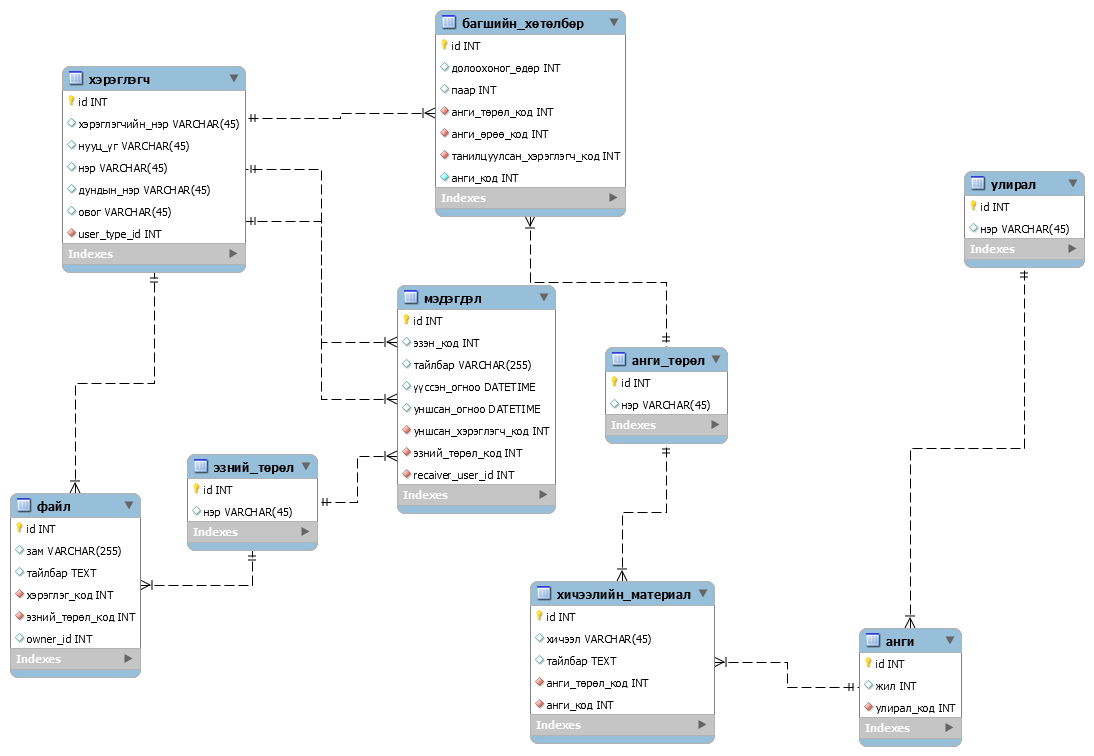
\includegraphics[scale=0.3]{Diagrams/S}
	\caption[ERD диаграм]{ERD диаграм}
	\label{fig:SClass}
\end{figure}

%--------------------------------------------------------------


\section{Үйл ажиллагааны диаграм}

\begin{figure}
	\centering
	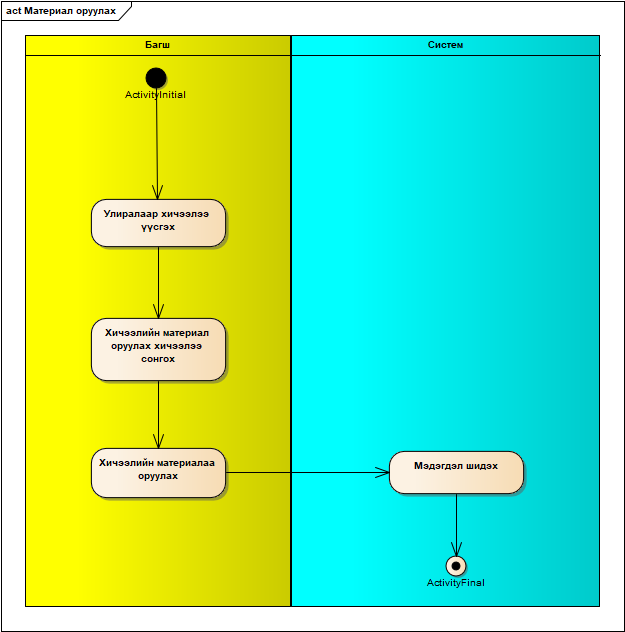
\includegraphics[angle=90, scale=0.7]{Diagrams/activity}
	\caption[Багш хичээлийн материал оруулах үйл ажиллагааны диаграм]{Багш хичээлийн материал оруулах үйл ажиллагааны диаграмм}
	\label{text}
\end{figure}
\newpage
\begin{figure}
	
	\centering
	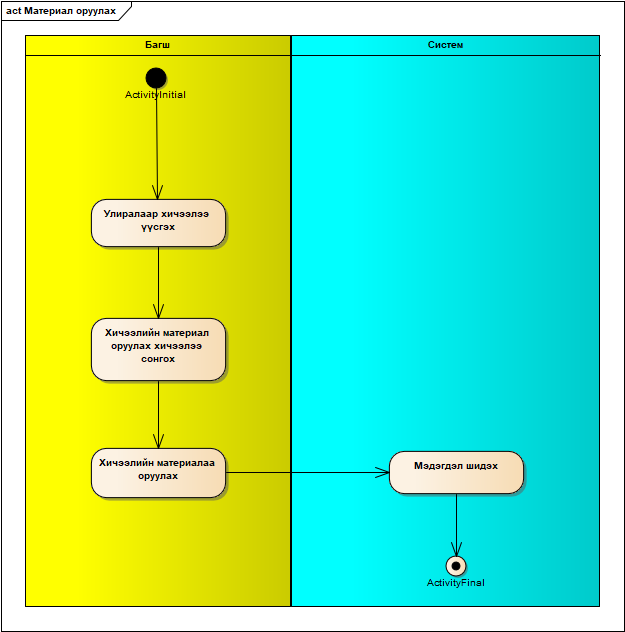
\includegraphics[angle=90, scale=0.75]{Diagrams/activity1}
	\caption[Багш тухайн хичээлийг үзэж байгаа оюутанг нэмэх үйл ажиллагааны диаграм]{Багш тухайн хичээлийг үзэж байгаа оюутанг нэмэх үйл ажиллагааны диаграм}
	\label{text}
\end{figure}

\newpage
\begin{figure}
	\centering
	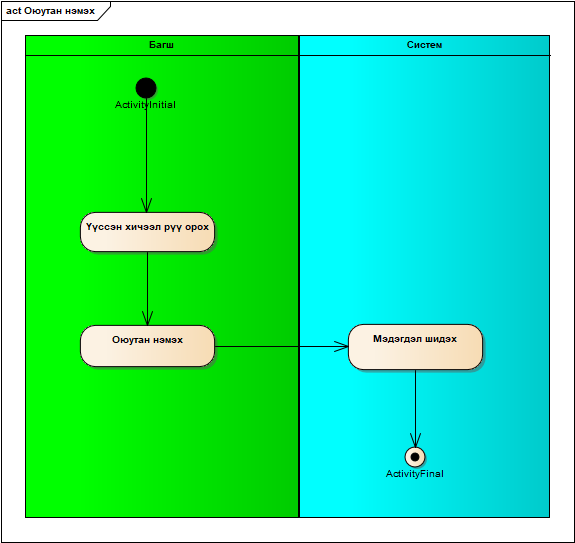
\includegraphics[angle=90, scale=0.8]{Diagrams/activity3}
	\caption[Оюутан хичээлийн материал татаж авах үйл ажиллагааны диаграм]{Оюутан хичээлийн материал татаж авах үйл ажиллагааны диаграм}
	\label{text}
\end{figure}

\newpage
\section{Дарааллын диаграм}
\newpage
\begin{figure}
	\centering
	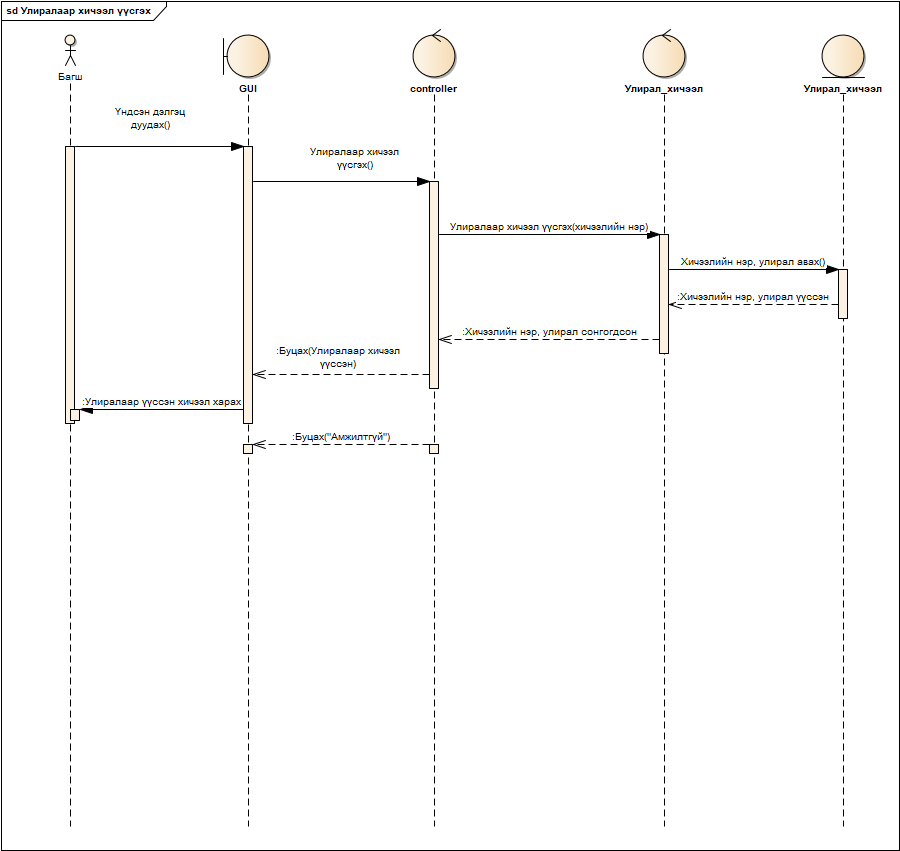
\includegraphics[angle=90, scale=0.5]{Diagrams/Sequence1}
	\caption[Багш улиралаар хичээл үүсгэх үйлдлийн дарааллын диаграм]{Багш улиралаар хичээл үүсгэх үйлдлийн дарааллын диаграм}
	\label{text}
\end{figure}

\newpage
\begin{figure}
	\centering
	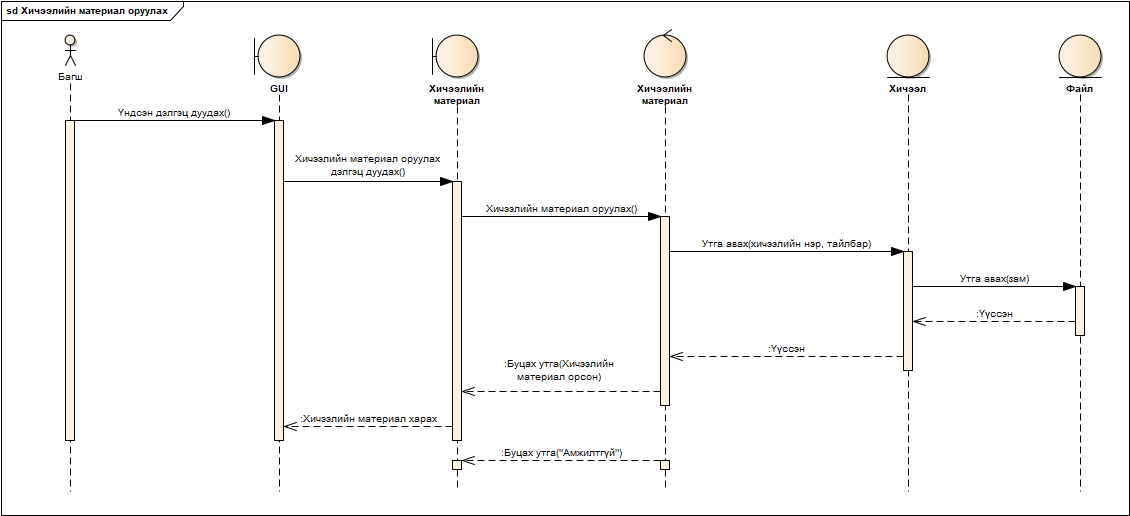
\includegraphics[angle=90, scale=0.5]{Diagrams/Sequence2}
	\caption[Багш хичээлийн материал оруулах үйлдлийн дарааллын диаграм]{Багш хичээлийн материал оруулах үйлдлийн дарааллын диаграм}
	\label{text}
\end{figure}

\newpage
\begin{figure}
	\centering
	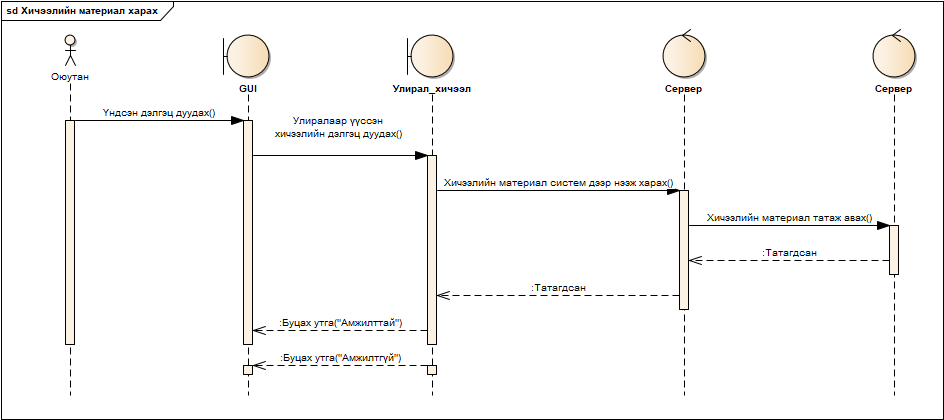
\includegraphics[angle=90, scale=0.5]{Diagrams/Sequence3}
	\caption[Оюутан хичээлийн материал татаж авах үйлдлийн дарааллын диаграм]{Оюутан хичээлийн материал татаж авах үйлдлийн дарааллын диаграм}
	\label{text}
\end{figure}

\newpage
\section{Класс диаграм}
\begin{figure}
	\centering
	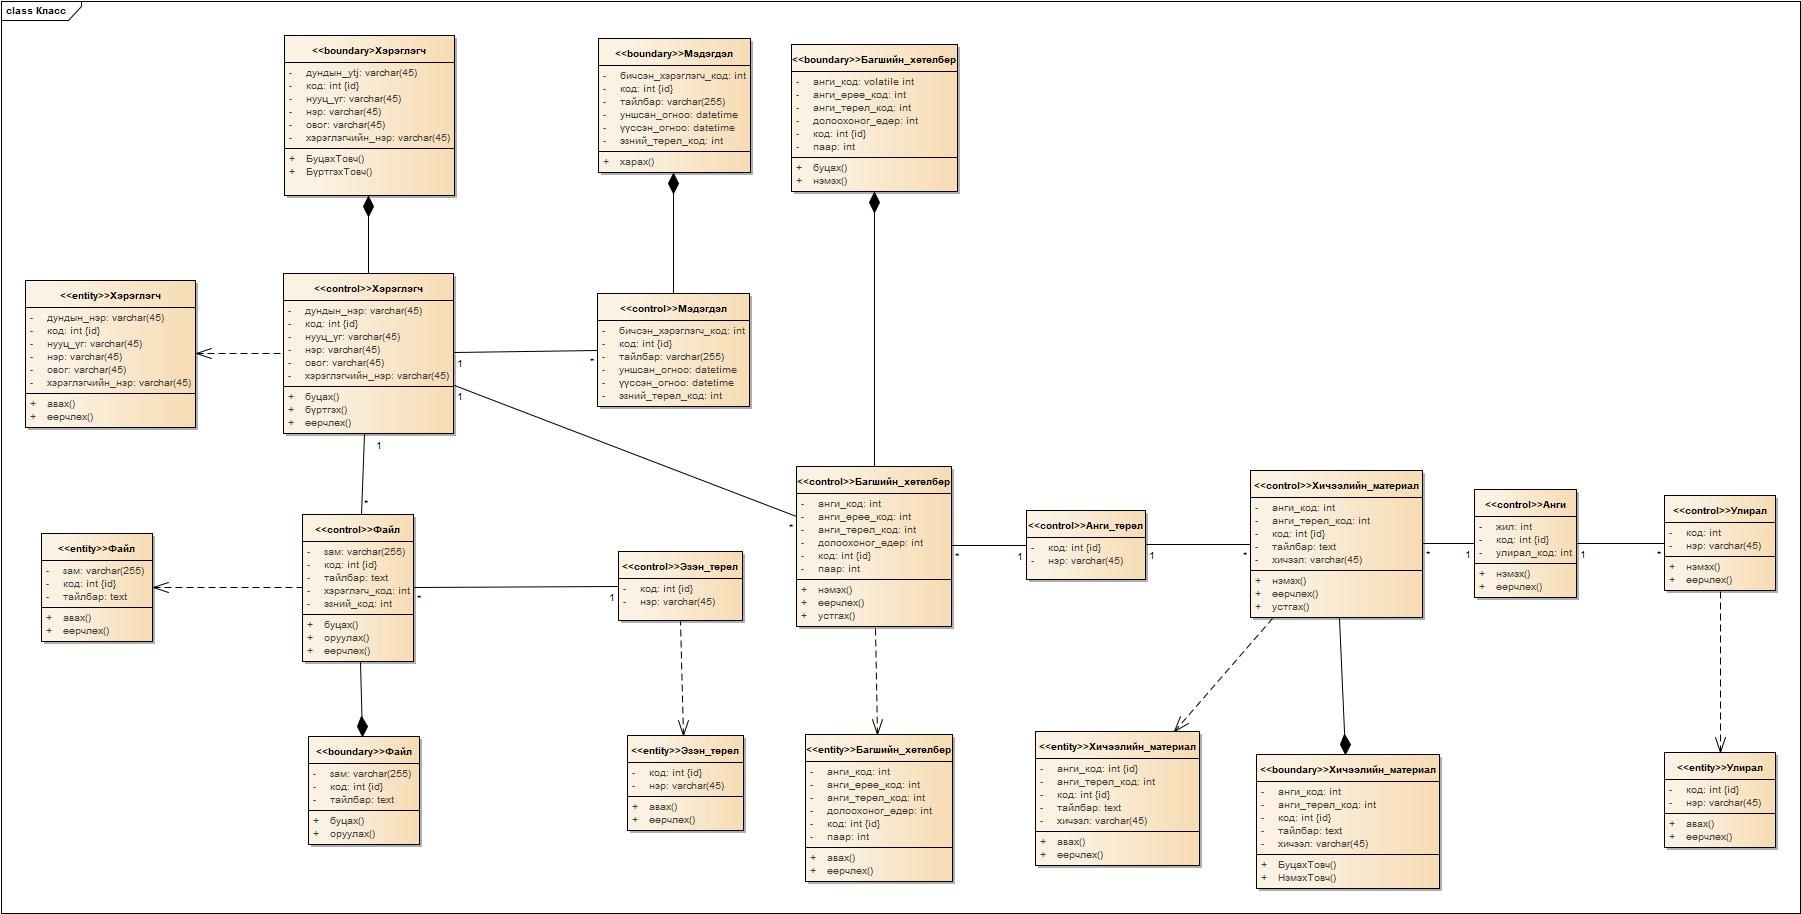
\includegraphics[angle=90, scale=0.4]{Diagrams/SClass}
	\caption[Класс диаграм]{Класс диаграм}
	\label{text}
\end{figure}

\newpage
\section{Бүлгийн дүгнэлт}
Хэрэглэгчийн шаардлагаа тодорхойлж тодорхойлсон шаардлага бүрээ нягтлан хянаж функционал болон фунционал бусаар нь ялгасан. Функционал шаардлага дээрээ үндэслэн юз кейс диаграмаа гаргасан ба бүх  юзкейс бүрт тодорхойлолт гаргасан. Мөн үйл ажиллагааны диаграм зурсан үйл ажиллагааг нь илүү нарийн ойлгомжтой болгож өгч байна.

 
	%% Бүлэг 3

\chapter{Системийн зохиомж} % Зарим нэг зөвлөмж
\label{Chapter3} % Энэ бүлэг рүү ишлэл хийх бол \ref{Chapter2} командыг ашигла 
\newpage
\section{Өгөгдлийн ерөнхий схем:}
		\begin{figure}[h!]
			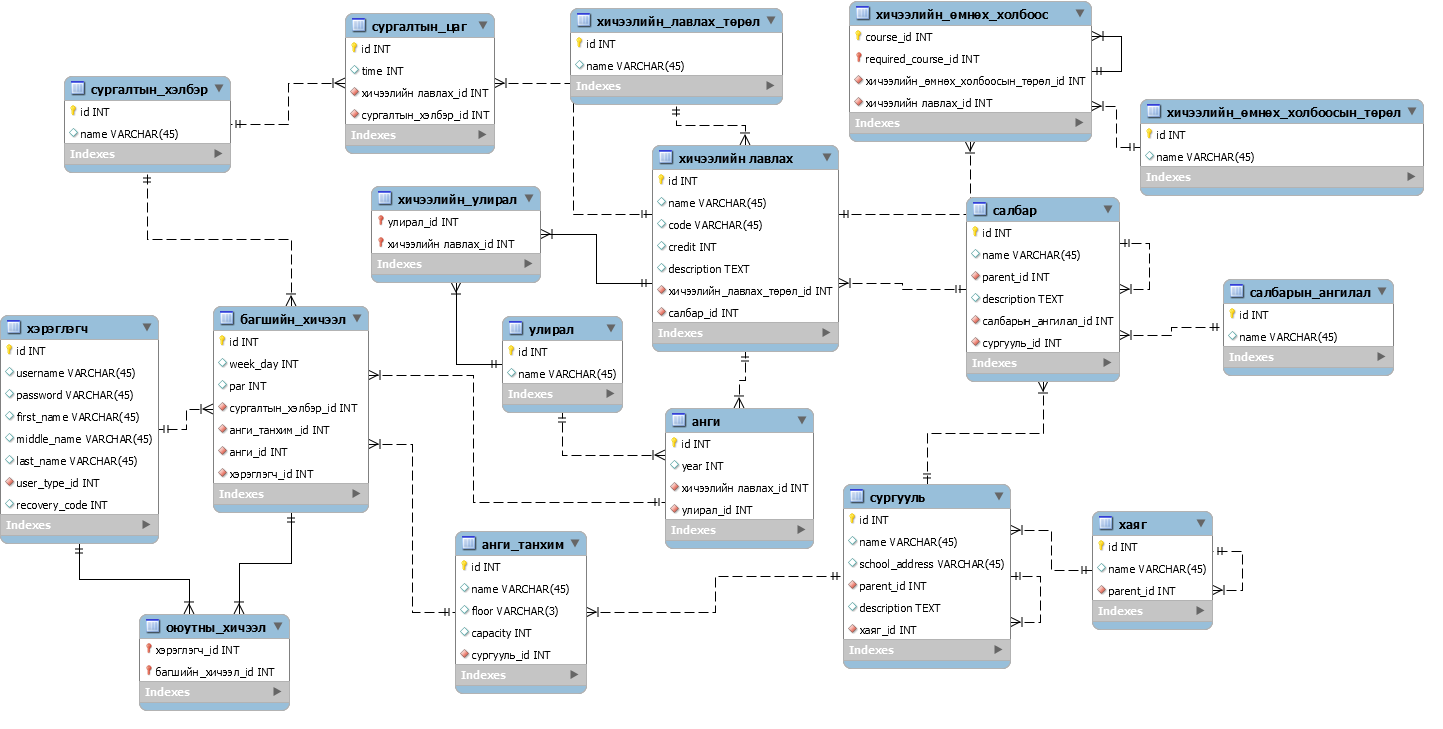
\includegraphics[angle=90, scale=0.4]{Diagrams/eschool_course}
			\caption[Өгөгдлийн ерөнхий схем]{Өгөгдлийн ерөнхий схем}
			\label{text}
		\end{figure}
\newpage	
\section{Класс диаграм}
	\begin{figure}[!h]
		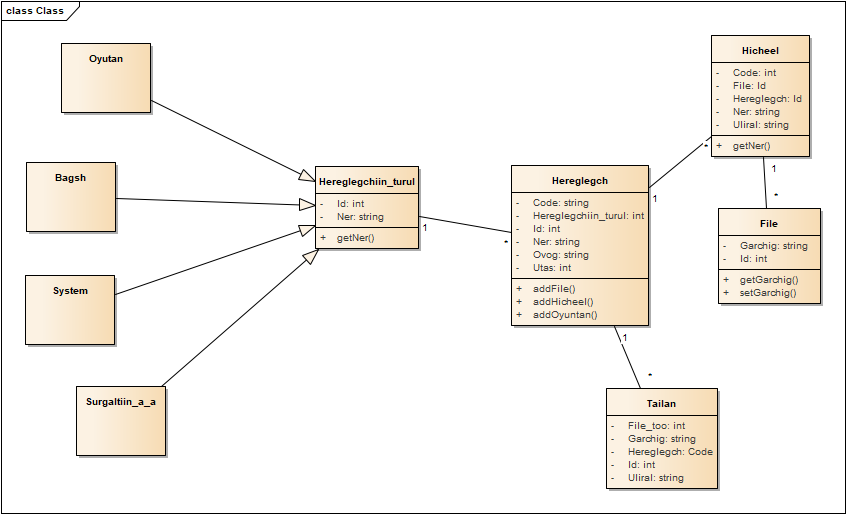
\includegraphics[angle=90,scale=0.5]{Diagrams/Class}
		\caption[Зохиомжийн шатны класс диаграм]{Зохиомжийн шатны класс диаграм}
		\label{text}
	\end{figure}
	
\newpage
\section{Хэрэглэгчийн интерфейс }

	\begin{figure}[!h]
		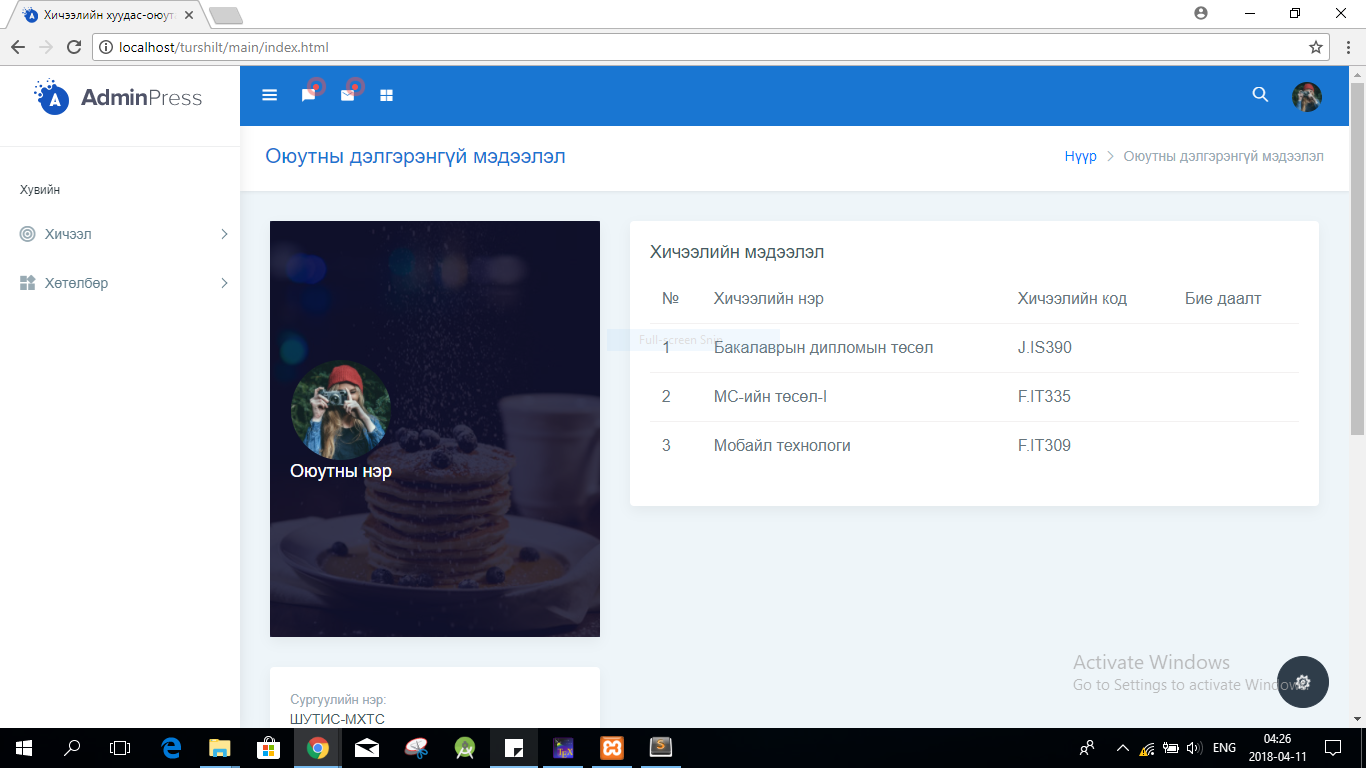
\includegraphics[scale=0.42]{Chart/screen-1}
		\caption[Оюутан харах нүүр хуудас]{Оюутан харах нүүр хуудас}
		\label{text}
	\end{figure}

	\begin{figure}[!h]
		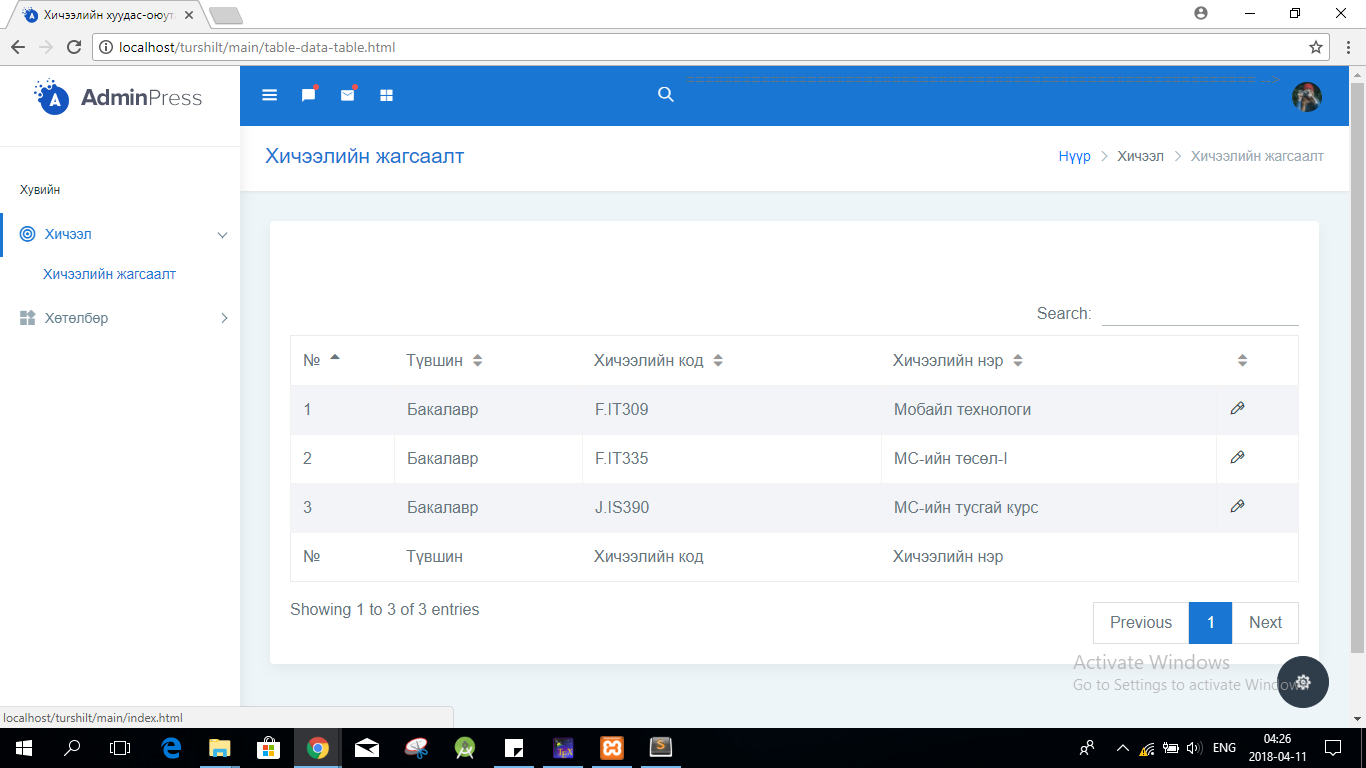
\includegraphics[scale=0.42]{Chart/screen-2}
		\caption[Оюутан хичээлийн жагсаалт харах]{Оюутан хичээлийн жагсаалт харах}
		\label{text}
	\end{figure}
	
	\begin{figure}[!h]
		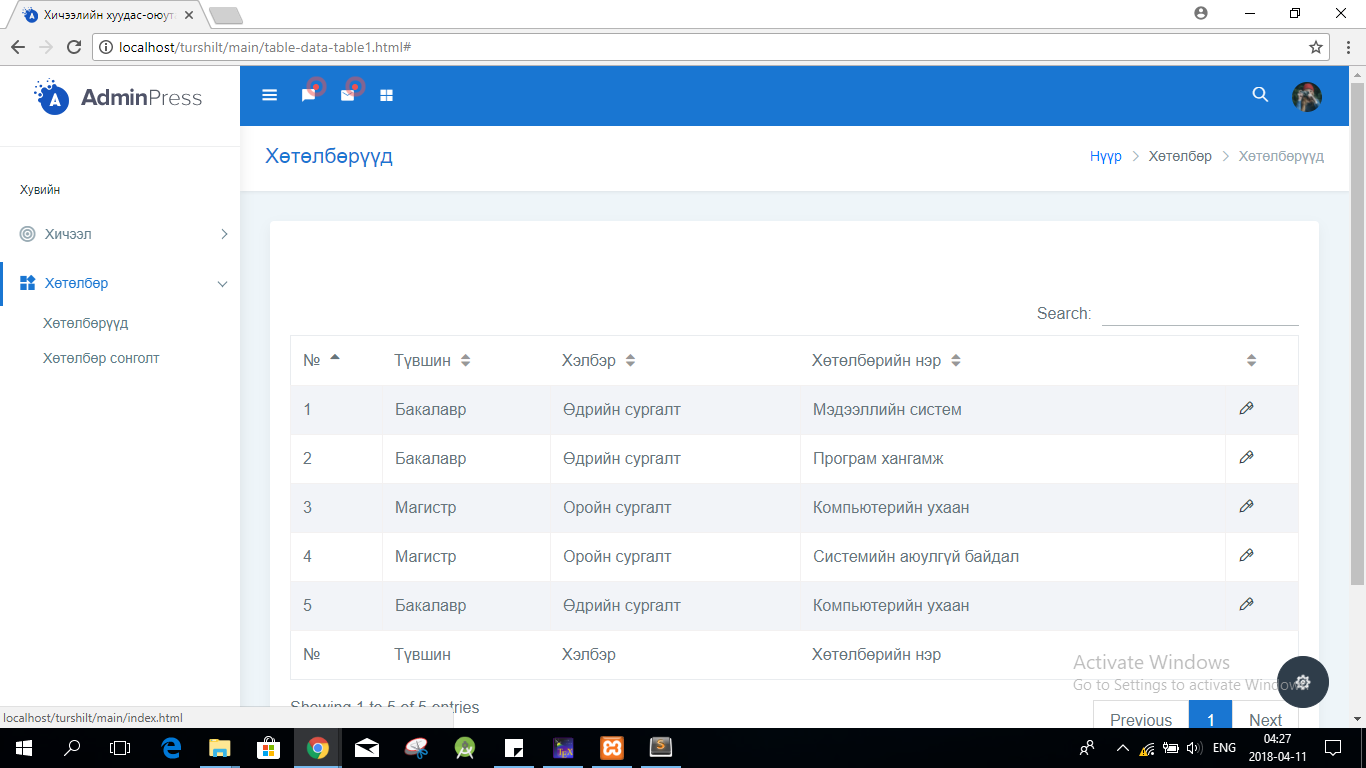
\includegraphics[scale=0.47]{Chart/screen-3}
		\caption[Оюутан хөтөлбөрийн мэдээлэл харах]{Оюутан хөтөлбөрийн мэдээлэл харах}
		\label{text}
	\end{figure}
	
	\begin{figure}[!h]
		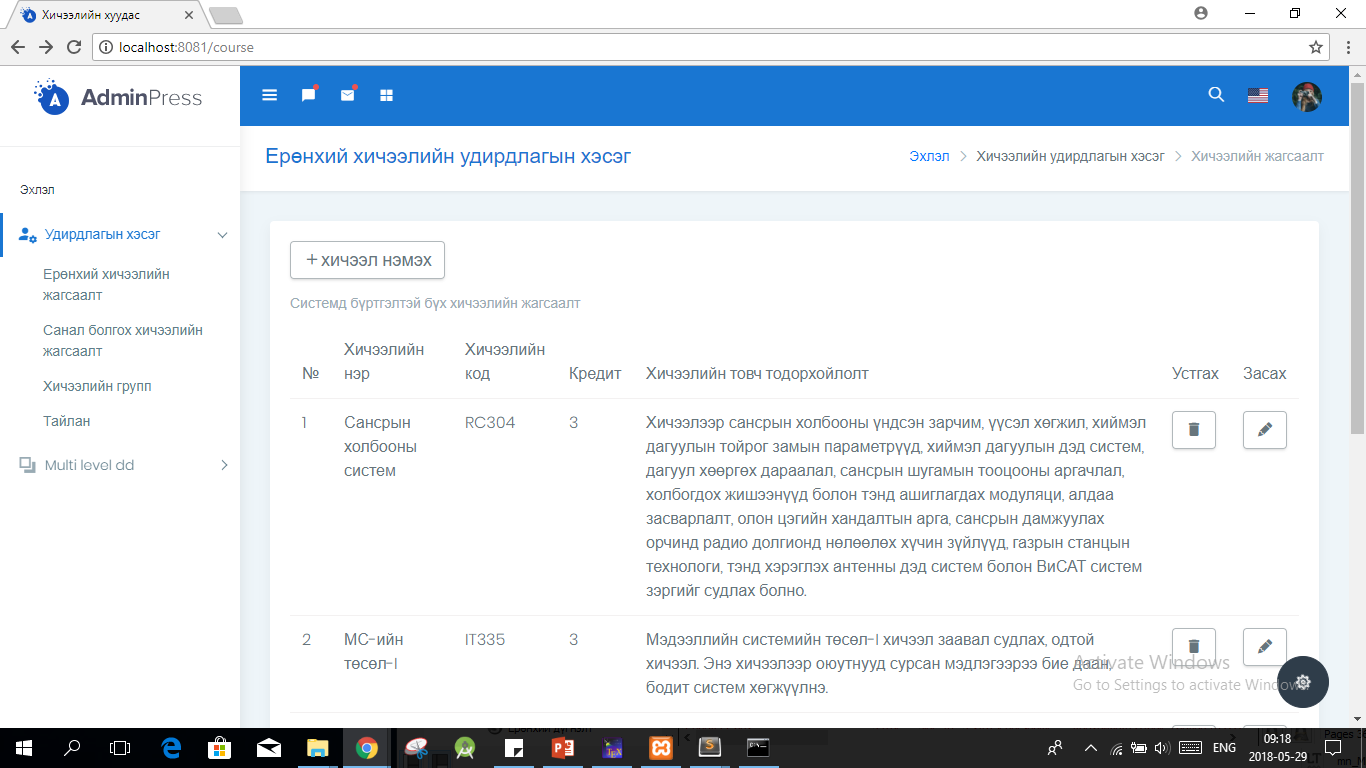
\includegraphics[scale=0.47]{Chart/screen-5}
		\caption[СА-ы ажилтан хичээл бүртгэх]{СА-ы ажилтан хичээл бүртгэх}
		\label{text}
	\end{figure}\begin{center}
	\begin{figure}[!h]
		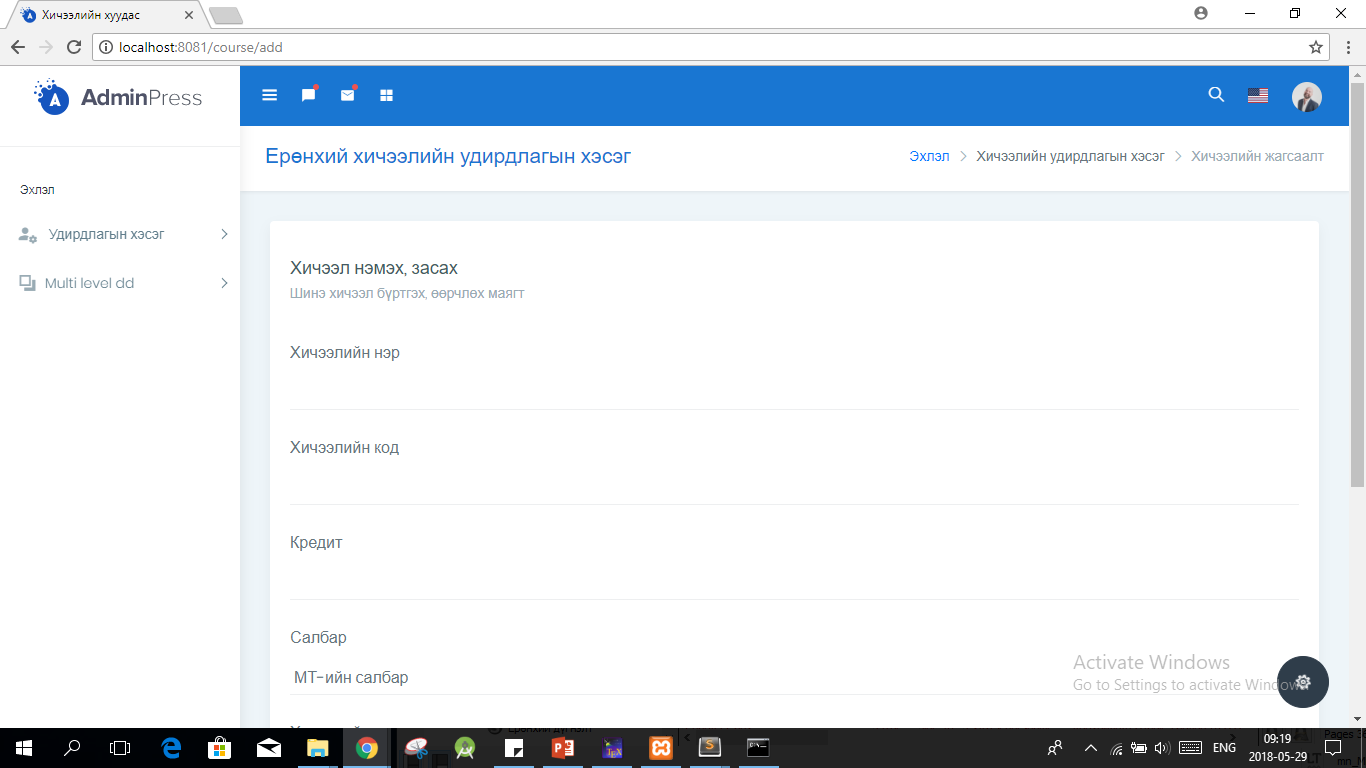
\includegraphics[scale=0.42]{Chart/screen-6}
		\caption[СА-ы ажилтан хичээл бүртгэх]{СА-ы ажилтан хичээл бүртгэх}
		\label{text}
	\end{figure}
\begin{figure}[!h]
	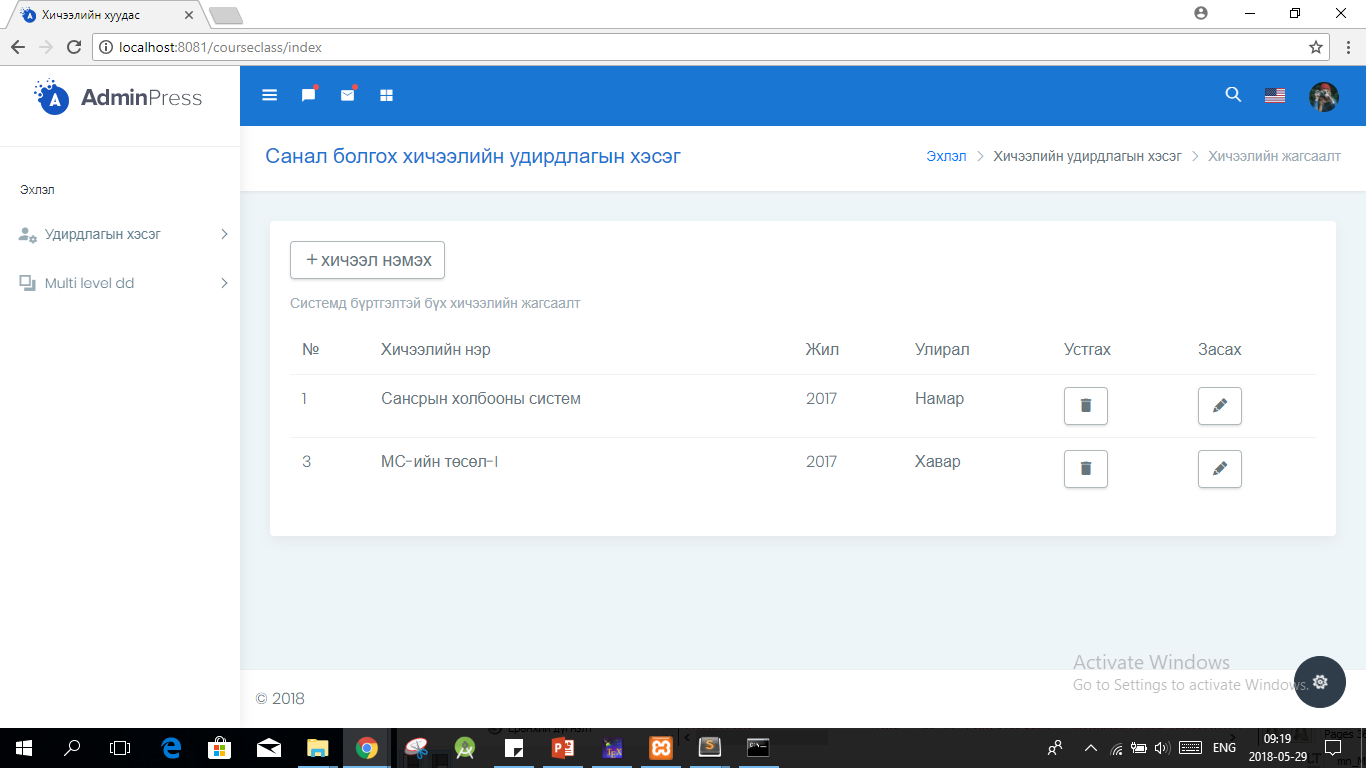
\includegraphics[scale=0.42]{Chart/screen-7}
	\caption[СА-ы ажилтан улирлын хичээл бүртгэх]{СА-ы ажилтан улирлын хичээл бүртгэх}
	\label{text}
\end{figure}
\begin{figure}[!h]
	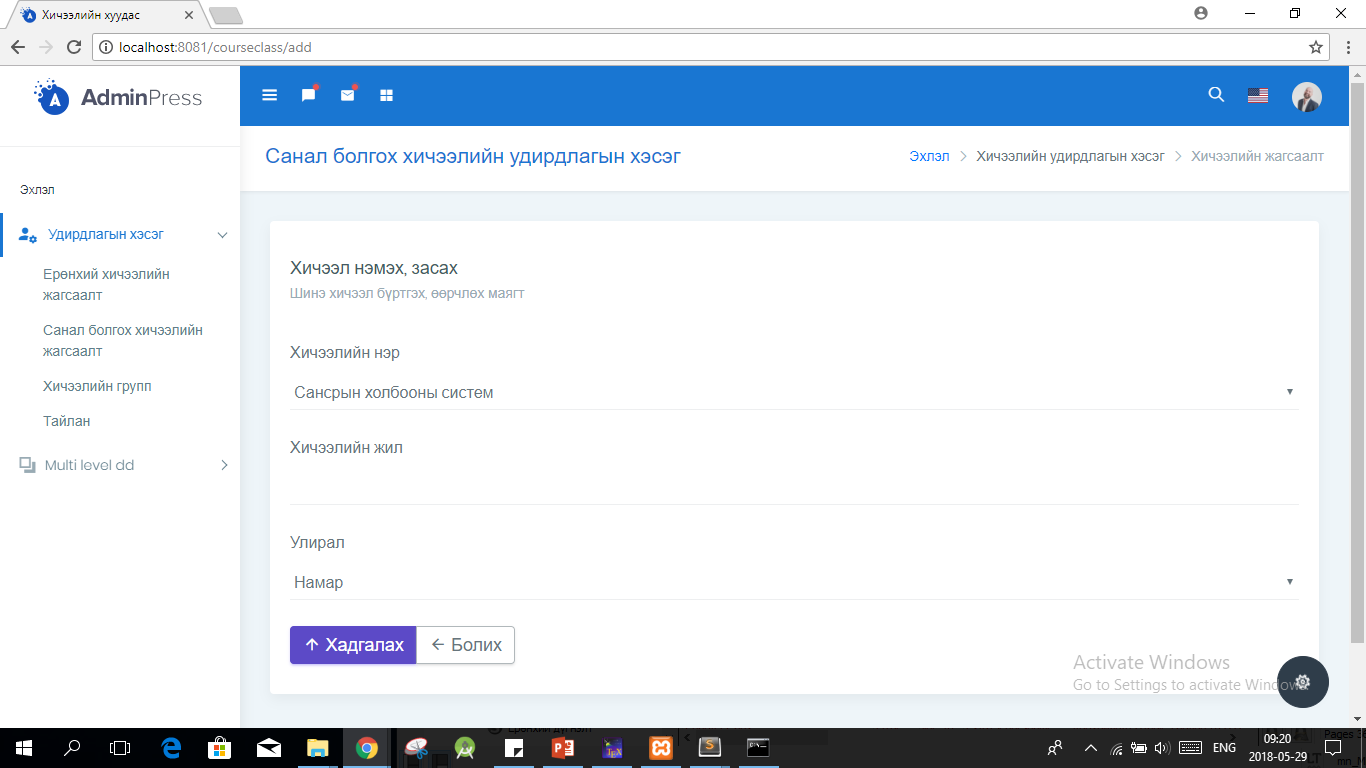
\includegraphics[scale=0.47]{Chart/screen-8}
	\caption[СА-ы ажилтан улирлын хичээл бүртгэх]{СА-ы ажилтан улирлын хичээл бүртгэх}
	\label{text}
\end{figure}
\begin{figure}[!h]
	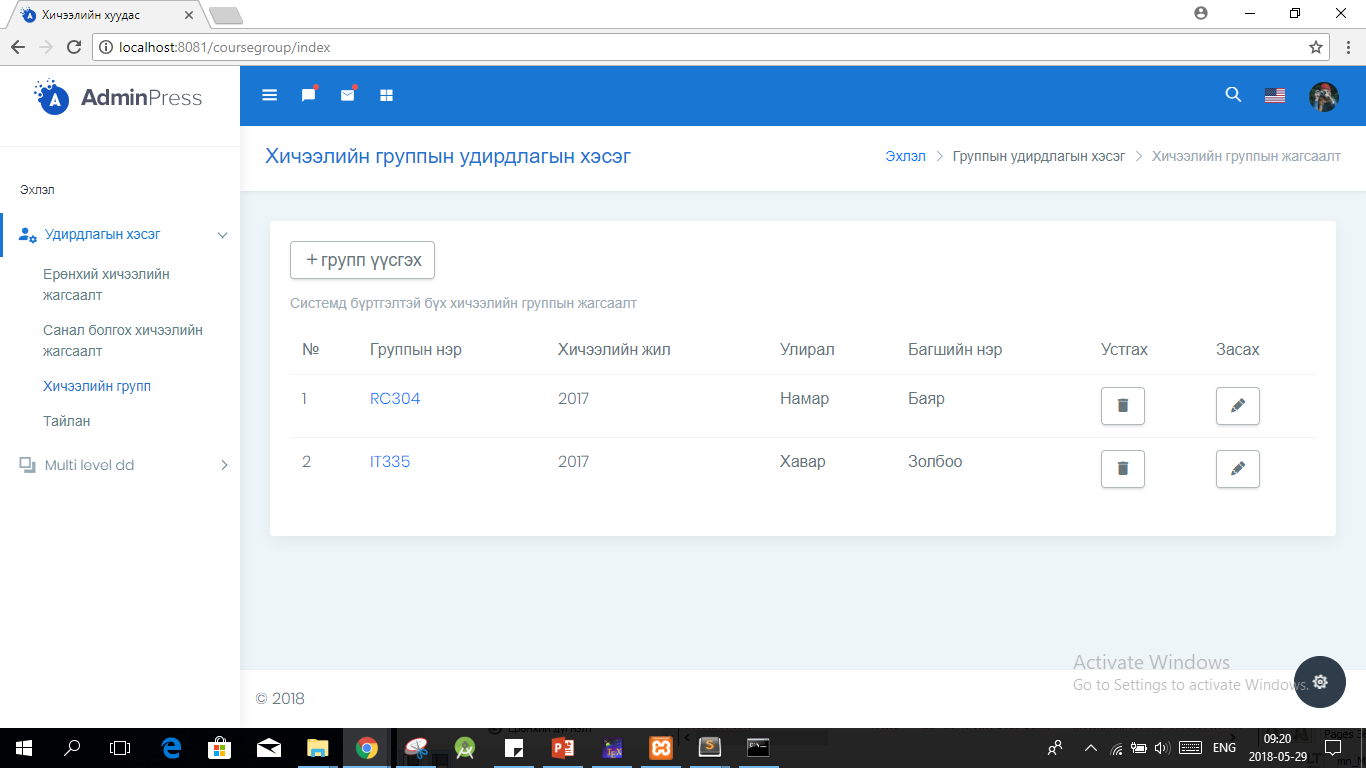
\includegraphics[scale=0.47]{Chart/screen-9}
	\caption[Групп үүсгэх]{Групп үүсгэх}
	\label{text}
\end{figure}
\begin{figure}[!h]
	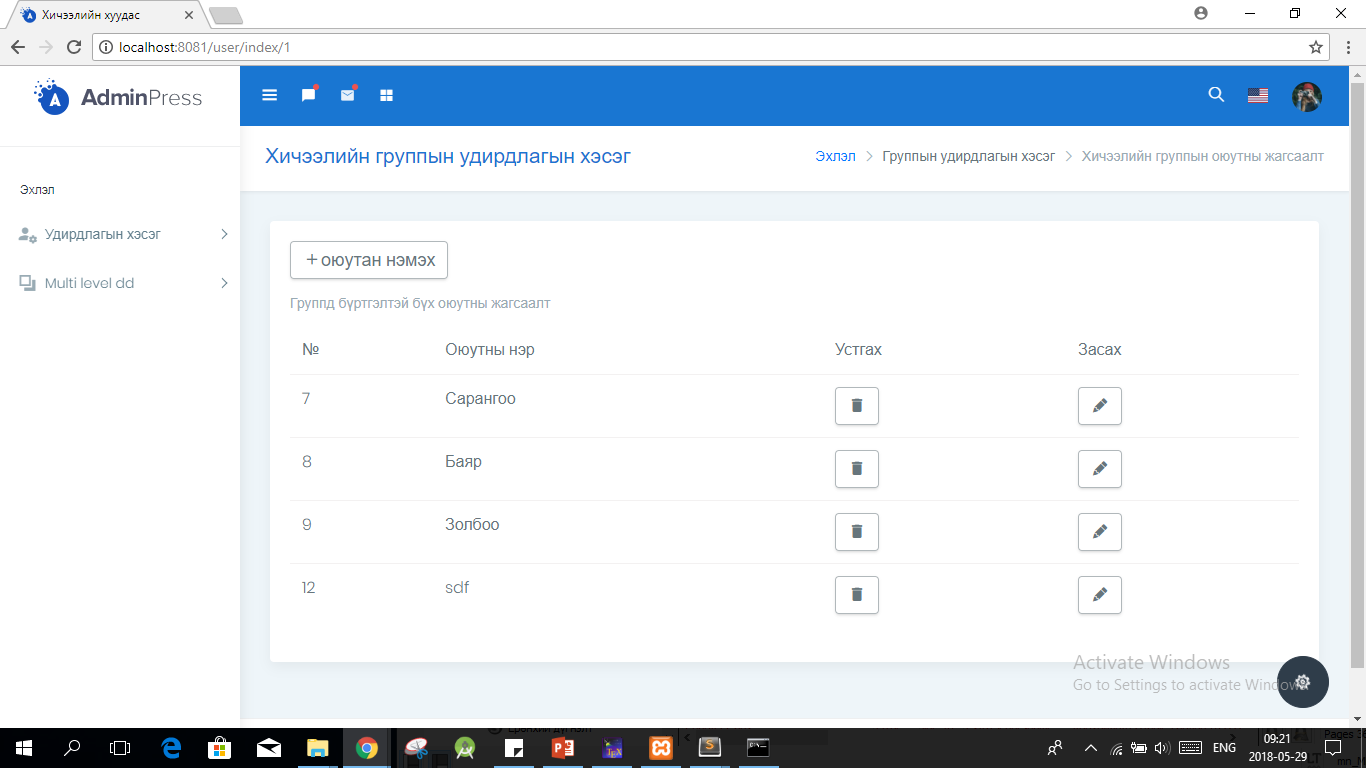
\includegraphics[scale=0.47]{Chart/screen-10}
	\caption[Групп-д гишүүн нэмэх]{Групп-д гишүүн нэмэх}
	\label{text}
\end{figure}
	
%\section{Тайлан, статистик үзүүлэлтийн загвар }
\newpage
\section{Бүлгийн дүгнэлт}
\hspace{1cm}Зохиомжийн хэсэгт өгөгдлийн ерөнхий схем болон өмнөх шинжилгээний класс диаграм дээр үндэслэн зохиомжийн класс диаграм, дарааллын диаграмуудыг гаргасан.
\section{Ерөнхий дүгнэлт}
\hspace{1cm}Мэдээллийн технологи хөгжиж байгаа энэ үед сургуульд хичээлийн веб хуудас үүсгэх нь суралцах зөв арга хэлбэр болж байна.\\
Энэхүү вебийг хийхэд дараах ажлуудыг хийж гүйцэтгэлээ:
\begin{itemize}
	\item Тухайн вебийн талаар судалгаа хийсэн.
	\item CodeIgniter framework –ийн судалгаа хийсэн.
	\item Өгөгдлийн сан болон вебийн дотоод үйл ажиллагааг дүрслэн гаргасан.
	\item Код бичих орчиноо бэлдэх, судалгаа шинжилгээ хийсэн.
\end{itemize}
	
	

	%\chapter{Ерөнхий дүгнэлт}

\section{Ерөнхий дүгнэлт}

	Энэ бүлэгт ... 
	%\include{Chapters/Chapter5}
	
	%-------------------------------------------------------------------------------
	%	THESIS CONTENT - APPENDICES
	%-------------------------------------------------------------------------------
	
	\appendix % Дараах "chapters" нь Хавсралт болохыг LaTex -д хэлэх
	
	% Тезисийн бүлгүүдийг Appendices хавтаснаас бие даасан файл байдлаар оруулах
	
%	% Хавсралт A

%\chapter{Хавсралтын нэр} % Main appendix title

\label{AppendixA} % For referencing this appendix elsewhere, use \ref{AppendixA}

Хавсралтаа энд бичнэ.Хавсралт шүү дараа нь хий
	%\include{Appendices/AppendixB}
	%\include{Appendices/AppendixC}
	
	%-------------------------------------------------------------------------------
	%	BIBLIOGRAPHY
	%-------------------------------------------------------------------------------
	\defformat % Бүлгийн нэрийг оргиналь байдлаар хэвлэх
	
	\addchaptertocentry{Ном зүй} % Ном зүйг гарчигт нэмэх
	
	\printbibliography[heading=bibliography,title={Ном зүй}]
	
	%-------------------------------------------------------------------------------
\end{document}
